%%%%%%%%%%%%%%%%%%%%%%%%%%%%%%%%%%%%%%%%%%%%%%%%%%%%%%%%%%%%%%%%%%%%%%%%%%%%
\def\TITLE{\bf フリーズパターン --- 数の繰返し模様の不思議}
\def\PDFTITLE{フリーズパターン 数の繰り返し模様の不思議}
\def\PDFAUTHOR{黒木玄}
\def\PDFSUBJECT{娯楽数学}
\def\AUTHOR{黒木玄}
\def\DATE{2013年7月7日%
\thanks{%
2013年7月7日: 第3.4版. $A^{(1)}_1$ 型の $K$ の定義の書き間違いを訂正した.
/ 2012年11月16日: 第3.3版. 湧き出し口と吸い込み口での変換の箙の図による説明を追加した.
/ 2012年11月14日: 第3.2版. \secref{sec:quiver-type}で $G_4$ を $G_2$ に訂正した.
/ 2012年11月12日: 第3.1版. \secref{sec:general-FP}の($*$)から上に3行目の
「頂点 $j$ から出る矢線」を「その頂点 $k$ から出る矢線」に訂正した.
/ 2012年11月8日: 第3.0版. 一般の型のフリーズパターンの解説を追加した.
/ 2012年9月5日: 第2.4版. hyperrefを使うようにした.
/ 2012年8月22日: 第2.3版. 微修正.
/ 2012年8月22日: 第2.2版. 
\problemref{problem:FF(t)}における $F(t)$ の定義を訂正した.
/ 2012年8月22日: 第2.1版. \secref{sec:A^{(1)}_1}と\secref{sec:A^{(2)}_2}
を大幅に訂正した. \secref{sec:triangulation}の位置を移動した.
/ 2012年8月20日: 第2.0版. \secref{sec:A^{(2)}_2}を追加.
/ 2012年8月17日: 第1.5版. \secref{sec:A^{(1)}_1}に $2$ 簡約の説明を追加.
/ 2012年8月17日: 第1.4版. \secref{sec:triangulation}の図を修正など.
/ 2012年8月16日: 第1.3版. 「単項式」を「係数 $1$ の単項式」に修正.
/ 2012年8月12日: 第1.2版.
/ 2012年8月10日: 第1.0版.}
\\ \href{http://www.math.tohoku.ac.jp/~kuroki/LaTeX/20120810FriezePattern.pdf}
{\small\tt http://www.math.tohoku.ac.jp/{\textasciitilde}kuroki/LaTeX/20120810FriezePattern.pdf}
%\thanks{
%この文書は仙台数学セミナー(2012年8月16日~18日に開催)のために作成された.
%仙台数学セミナーは, ジブラルタ生命保険株式会社と
%東北大学大学院理学研究科数学専攻の協賛のもとで
%川井数理科学財団によって毎年開催されており, 
%夏休みのあいだに高校生に仙台に来てもらって数学の話を聴いてもらっている.
%川井財団のウェブサイトが次の場所にある: 
%{\tt http://morpho.sci.tohoku.ac.jp/{\textasciitilde}kawai/}}
}
%%%%%%%%%%%%%%%%%%%%%%%%%%%%%%%%%%%%%%%%%%%%%%%%%%%%%%%%%%%%%%%%%%%%%%%%%%%%
\documentclass[12pt,twoside,dvipdfm]{jarticle}
\usepackage{amsmath,amssymb,amsthm}
%%%%%%%%%%%%%%%%%%%%%%%%%%%%%%%%%%%%%%%%%%%%%%%%%%%%%%%%%%%%%%%%%%%%%%%%%%%%%%
%\usepackage{hyperref}
\usepackage[dvipdfmx]{hyperref}
\usepackage{pxjahyper}
\hypersetup{%
 bookmarksnumbered=true,%
 colorlinks=true,%
 setpagesize=false,%
 pdftitle={\PDFTITLE},%
 pdfauthor={\PDFAUTHOR},%
 pdfsubject={\PDFSUBJECT},%
 pdfkeywords={TeX; dvipdfmx; hyperref; color;}}
\newcommand\arxivref[1]{\href{http://arxiv.org/abs/#1}{\tt arXiv:#1}}
\newcommand\TILDE{\textasciitilde}
\newcommand\US{\textunderscore}
%%%%%%%%%%%%%%%%%%%%%%%%%%%%%%%%%%%%%%%%%%%%%%%%%%%%%%%%%%%%%%%%%%%%%%%%%%%%%%
\usepackage[dvipdfm]{graphicx}
\usepackage[all]{xy}
%%%%%%%%%%%%%%%%%%%%%%%%%%%%%%%%%%%%%%%%%%%%%%%%%%%%%%%%%%%%%%%%%%%%%%%%%%%%%%
\pagestyle{plain}
\setlength{\oddsidemargin}{0cm}
\setlength{\evensidemargin}{0cm}
\setlength{\topmargin}{-1.3cm}
\setlength{\textheight}{25cm}
\setlength{\textwidth}{16cm}
\allowdisplaybreaks
%%%%%%%%%%%%%%%%%%%%%%%%%%%%%%%%%%%%%%%%%%%%%%%%%%%%%%%%%%%%%%%%%%%%%%%%%%%%%%
\usepackage[dvipdfm]{color}
\newcommand\red{\color{red}}
\newcommand\blue{\color{blue}}
\newcommand\green{\color{green}}
\newcommand\magenta{\color{magenta}}
\newcommand\cyan{\color{cyan}}
\newcommand\yellow{\color{yellow}}
\newcommand\white{\color{white}}
\newcommand\black{\color{black}}
\renewcommand\r{\red}
\renewcommand\b{\blue}
%%%%%%%%%%%%%%%%%%%%%%%%%%%%%%%%%%%%%%%%%%%%%%%%%%%%%%%%%%%%%%%%%%%%%%%%%%%%
\makeatletter
  \def\Ddots{\mathinner{\mkern1mu
      \raise\p@\hbox{.}\mkern2mu\raise4\p@\hbox{.}\mkern2mu
      \raise7\p@\vbox{\kern7\p@\hbox{.}}\mkern1mu}}
  \makeatother
%%%%%%%%%%%%%%%%%%%%%%%%%%%%%%%%%%%%%%%%%%%%%%%%%%%%%%%%%%%%%%%%%%%%%%%%%%%%
%\newcommand\N{{\mathbb N}} % natural numbers
\newcommand\Z{{\mathbb Z}} % rational integers
\newcommand\F{{\mathbb F}} % finite field
\newcommand\Q{{\mathbb Q}} % rational numbers
\newcommand\R{{\mathbb R}} % real numbers
\newcommand\C{{\mathbb C}} % complex numbers
%\renewcommand\P{{\mathbb P}} % projective spaces
%%%%%%%%%%%%%%%%%%%%%%%%%%%%%%%%%%%%%%%%%%%%%%%%%%%%%%%%%%%%%%%%%%%%%%%%%%%%
%
% 定理環境
%
%\theoremstyle{plain} % 見出しをボールド、本文で斜体を使う
\theoremstyle{definition} % 見出しをボールド、本文で斜体を使わない
\newtheorem{theorem}{定理}
\newtheorem*{theorem*}{定理} % 番号を付けない
\newtheorem{prop}[theorem]{命題}
\newtheorem*{prop*}{命題}
\newtheorem{lemma}[theorem]{補題}
\newtheorem*{lemma*}{補題}
\newtheorem{cor}[theorem]{系}
\newtheorem*{cor*}{系}
\newtheorem{example}[theorem]{例}
\newtheorem*{example*}{例}
\newtheorem{axiom}[theorem]{公理}
\newtheorem*{axiom*}{公理}
\newtheorem{problem}[theorem]{問題}
\newtheorem*{problem*}{問題}
\newtheorem{summary}[theorem]{要約}
\newtheorem*{summary*}{要約}
\newtheorem{guide}[theorem]{参考}
\newtheorem*{guide*}{参考}
%
\theoremstyle{definition} % 見出しをボールド、本文で斜体を使わない
\newtheorem{definition}[theorem]{定義}
\newtheorem*{definition*}{定義} % 番号を付けない
%
%\theoremstyle{remark} % 見出しをイタリック、本文で斜体を使わない
\theoremstyle{definition} % 見出しをボールド、本文で斜体を使わない
\newtheorem{remark}[theorem]{注意}
\newtheorem*{remark*}{注意}
%
\numberwithin{theorem}{section}
\numberwithin{equation}{section}
\numberwithin{figure}{section}
\numberwithin{table}{section}
%
% 引用コマンド
%
\newcommand\secref[1]{第\ref{#1}節}
\newcommand\theoremref[1]{定理\ref{#1}}
\newcommand\propref[1]{命題\ref{#1}}
\newcommand\lemmaref[1]{補題\ref{#1}}
\newcommand\corref[1]{系\ref{#1}}
\newcommand\exampleref[1]{例\ref{#1}}
\newcommand\axiomref[1]{公理\ref{#1}}
\newcommand\problemref[1]{問題\ref{#1}}
\newcommand\summaryref[1]{要約\ref{#1}}
\newcommand\guideref[1]{参考\ref{#1}}
\newcommand\definitionref[1]{定義\ref{#1}}
\newcommand\remarkref[1]{注意\ref{#1}}
%
\newcommand\figureref[1]{図\ref{#1}}
\newcommand\figref[1]{\figureref{#1}}
\newcommand\tableref[1]{表\ref{#1}}
%
% \qed を自動で入れない proof 環境を再定義
%
\makeatletter
\renewenvironment{proof}[1][\proofname]{\par
%\newenvironment{Proof}[1][\Proofname]{\par
  \normalfont
  \topsep6\p@\@plus6\p@ \trivlist
  \item[\hskip\labelsep{\bfseries #1}\@addpunct{\bfseries.}]\ignorespaces
}{%
  \endtrivlist
}
\renewcommand{\proofname}{証明}
%\newcommand{\Proofname}{証明}
\makeatother
%
% 正方形の \qed を長方形に再定義
%
\makeatletter
\def\BOXSYMBOL{\RIfM@\bgroup\else$\bgroup\aftergroup$\fi
  \vcenter{\hrule\hbox{\vrule height.85em\kern.6em\vrule}\hrule}\egroup}
\makeatother
\newcommand{\BOX}{%
  \ifmmode\else\leavevmode\unskip\penalty9999\hbox{}\nobreak\hfill\fi
  \quad\hbox{\BOXSYMBOL}}
\renewcommand\qed{\BOX}
%\newcommand\QED{\BOX}
%%%%%%%%%%%%%%%%%%%%%%%%%%%%%%%%%%%%%%%%%%%%%%%%%%%%%%%%%%%%%%%%%%%%%%%%%%%%
\begin{document}
%%%%%%%%%%%%%%%%%%%%%%%%%%%%%%%%%%%%%%%%%%%%%%%%%%%%%%%%%%%%%%%%%%%%%%%%%%%%
\title{\TITLE}
\author{\AUTHOR}
\date{\DATE}
\maketitle
\tableofcontents
%%%%%%%%%%%%%%%%%%%%%%%%%%%%%%%%%%%%%%%%%%%%%%%%%%%%%%%%%%%%%%%%%%%%%%%%%%%%
%\setcounter{section}{-1} % 最初の節番号を0にする

\section{Conway-Coxeterのフリーズパターン ($A$ 型の場合)}

\begin{figure}[ht]%[htbp!]
\begin{center}
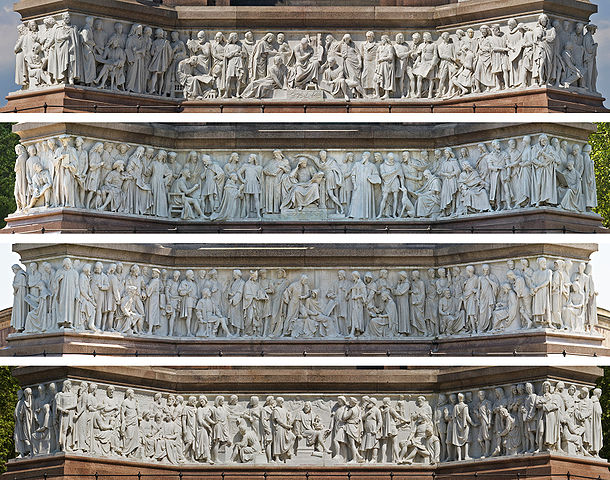
\includegraphics[width=14cm]{610px-Albert_Memorial_Friese_Collage_-_May_2008-edit1.jpg}
\caption{Frieze of Parnassus.
Photo by DAVID ILIFF. License: CC-BY-SA 3.0. \newline
\href{http://en.wikipedia.org/wiki/Frieze_of_Parnassus}
{\tt http://en.wikipedia.org/wiki/Frieze\_of\_Parnassus}
}
\label{fig:frieze1}
\end{center}
\end{figure}

数学の世界ではとても不思議な面白い法則が成立していることがよくある.

このノートではその実例としてフリーズパターン(frieze pattern)について紹介したい.
フリーズパターンは簡単なルールに基いて作られる数が並んでいる様子のことである.
フリーズパターンを生成するためのルールは一通りではない.

フリーズパターン生成のルールをある種のものに限ると
フリーズパターンは繰返し模様になる.
その様子が装飾された横壁(\figureref{fig:frieze1})
の様子に似ているのでそれを表わす frieze (フリーズ)
という名前が付いているのだろう.

最も簡単なルールで生成されるフリーズパターンは 
Conway-Coxeter (コンウェイ・コクセター)のフリーズパターンと呼ばれている.
Conway-Coxeter のフリーズパターンは
次のようにひし形に並べられた数 $a,b,c,d$ が $ad=bc+1$
という規則を満たすという条件で生成される:
\begin{equation*}
\begin{array}{ccc}
   & b &   \\
 a &   & d \\
   & c &   \\
\end{array}
\qquad\qquad
ad = bc+1.
\end{equation*} 
$a,b,c$ から $d$ を $d = (bc+1)/a$ によって決めることができる%
\footnote{$A/B$ は $A$ を $B$ で割る演算を表わしている.}.
(逆に $b,c,d$ から $a$ を $a=(bc+1)/d$ によって決めることもできる.)

このことを使えば, たとえば最初に次のように $1$ を並べた状況から出発して
最上段と最下段の $1$ の並びのあいだの空いている部分をすべて埋めることができる:
\begin{equation*}
\begin{array}{cccccccccccccccccccc}
   &   & 1 &   & 1 &   & 1 &   & 1 &   & 1 &   & 1 &   & 1 &   & 1 &   &   &   \\ \hline
   & 1 &   &   &   &   &   &   &   &   &   &   &   &   &   &   &   &   &   &   \\
 1 &   &   &   &   &   &   &   &   &   &   &   &   &   &   &   &   &   &   &   \\
   & 1 &   &   &   &   &   &   &   &   &   &   &   &   &   &   &   &   &   &   \\
   &   & 1 &   &   &   &   &   &   &   &   &   &   &   &   &   &   &   &   &   \\
   &   &   & 1 &   &   &   &   &   &   &   &   &   &   &   &   &   &   &   &   \\ \hline
   &   &   &   & 1 &   & 1 &   & 1 &   & 1 &   & 1 &   & 1 &   & 1 &   & 1 &   \\
\end{array}
\end{equation*}
左から右に空いている部分を埋めていってみよう.
最初のステップは次の通り:
\begin{align*}
&
\begin{array}{cccccccccccccccccccc}
    &   & 1 &   & 1 &   & 1 &   & 1 &   & 1 &   & 1 &   & 1 &   & 1 &   &   &   \\ \hline
    &\b1&   &   &   &   &   &   &   &   &   &   &   &   &   &   &   &   &   &   \\
 \b1&   &\r2&   &   &   &   &   &   &   &   &   &   &   &   &   &   &   &   &   \\
    &\b1&   &   &   &   &   &   &   &   &   &   &   &   &   &   &   &   &   &   \\
    &   & 1 &   &   &   &   &   &   &   &   &   &   &   &   &   &   &   &   &   \\
    &   &   & 1 &   &   &   &   &   &   &   &   &   &   &   &   &   &   &   &   \\ \hline
    &   &   &   & 1 &   & 1 &   & 1 &   & 1 &   & 1 &   & 1 &   & 1 &   & 1 &   \\
\end{array}
\\[\bigskipamount] & \quad
({\b1}\times{\b1}+1)/{\b1}={\r2}
\end{align*} 
左端の $a=1$, $b=1$, $c=1$ から $d=(bc+1)/a=2$ を計算した.
この手続きを同様に繰返す. 次のステップ:
\begin{align*}
&
\begin{array}{cccccccccccccccccccc}
    &   &\b1&   & 1 &   & 1 &   & 1 &   & 1 &   & 1 &   & 1 &   & 1 &   &   &   \\ \hline
    &\b1&   &\r3&   &   &   &   &   &   &   &   &   &   &   &   &   &   &   &   \\
  1 &   &\b2&   &   &   &   &   &   &   &   &   &   &   &   &   &   &   &   &   \\
    &\b1&   &\r3&   &   &   &   &   &   &   &   &   &   &   &   &   &   &   &   \\
    &   &\b1&   &   &   &   &   &   &   &   &   &   &   &   &   &   &   &   &   \\
    &   &   & 1 &   &   &   &   &   &   &   &   &   &   &   &   &   &   &   &   \\ \hline
    &   &   &   & 1 &   & 1 &   & 1 &   & 1 &   & 1 &   & 1 &   & 1 &   & 1 &   \\
\end{array}
\\[\bigskipamount] & \quad
({\b1}\times{\b2}+1)/{\b1}={\r3}
\\ & \quad
({\b2}\times{\b1}+1)/{\b1}={\r3}
\end{align*} 
さらに次のステップ:
\begin{align*}
&
\begin{array}{cccccccccccccccccccc}
    &   & 1 &   & 1 &   & 1 &   & 1 &   & 1 &   & 1 &   & 1 &   & 1 &   &   &   \\ \hline
    & 1 &   &\b3&   &   &   &   &   &   &   &   &   &   &   &   &   &   &   &   \\
  1 &   &\b2&   &\r5&   &   &   &   &   &   &   &   &   &   &   &   &   &   &   \\
    & 1 &   &\b3&   &   &   &   &   &   &   &   &   &   &   &   &   &   &   &   \\
    &   &\b1&   &\r4&   &   &   &   &   &   &   &   &   &   &   &   &   &   &   \\
    &   &   &\b1&   &   &   &   &   &   &   &   &   &   &   &   &   &   &   &   \\ \hline
    &   &   &   & 1 &   & 1 &   & 1 &   & 1 &   & 1 &   & 1 &   & 1 &   & 1 &   \\
\end{array}
\\[\bigskipamount] & \quad
({\b3}\times{\b3}+1)/{\b2}={\r5}
\\ & \quad
({\b3}\times{\b1}+1)/{\b1}={\r4}
\\ & \quad
\phantom{({\b2}\times{\b1}+1)/{\b1}={\r3}}
\end{align*}
さらに次のステップ:
\begin{align*}
&
\begin{array}{cccccccccccccccccccc}
    &   & 1 &   &\b1&   & 1 &   & 1 &   & 1 &   & 1 &   & 1 &   & 1 &   &   &   \\ \hline
    & 1 &   &\b3&   &\r2&   &   &   &   &   &   &   &   &   &   &   &   &   &   \\
  1 &   & 2 &   &\b5&   &   &   &   &   &   &   &   &   &   &   &   &   &   &   \\
    & 1 &   &\b3&   &\r7&   &   &   &   &   &   &   &   &   &   &   &   &   &   \\
    &   & 1 &   &\b4&   &   &   &   &   &   &   &   &   &   &   &   &   &   &   \\
    &   &   &\b1&   &\r5&   &   &   &   &   &   &   &   &   &   &   &   &   &   \\ \hline
    &   &   &   &\b1&   & 1 &   & 1 &   & 1 &   & 1 &   & 1 &   & 1 &   & 1 &   \\
\end{array}
\\[\bigskipamount] & \quad
({\b1}\times{\b5}+1)/{\b3}={\r2}
\\ & \quad
({\b5}\times{\b4}+1)/{\b3}={\r7}
\\ & \quad
({\b4}\times{\b1}+1)/{\b1}={\r5}
\end{align*} 
同様に計算を続けると次のようになることがわかる:
\begin{equation*}
\begin{array}{cccccccccccccccccccc}
    &   & 1 &   & 1 &   & 1 &   & 1 &   & 1 &   & 1 &   & 1 &   & 1 &   &   &   \\ \hline
    &\b1&   & 3 &   & 2 &   & 2 &   & 2 &   &\r1&   &   &   &   &   &   &   &   \\
 \b1&   & 2 &   & 5 &   & 3 &   & 3 &   &\r1&   &   &   &   &   &   &   &   &   \\
    &\b1&   & 3 &   & 7 &   & 4 &   &\r1&   &   &   &   &   &   &   &   &   &   \\
    &   &\b1&   & 4 &   & 9 &   &\r1&   &   &   &   &   &   &   &   &   &   &   \\
    &   &   &\b1&   & 5 &   & 2 &   &\r1&   &   &   &   &   &   &   &   &   &   \\ \hline
    &   &   &   & 1 &   & 1 &   & 1 &   & 1 &   & 1 &   & 1 &   & 1 &   & 1 &   \\
\end{array}
\end{equation*}
赤い $\r1$ の部分は青い $\b1$ の上下をひっくり返した形になっている. \\
Conway-Coxeter のフリーズパターンのルールは上下を反転しても変わらない. \\
したがって, 残りの部分は同じパターンの繰り返しになる:
\begin{equation}
\begin{array}{cccccccccccccccccccc}
   &   & 1 &   & 1 &   & 1 &   & 1 &   & 1 &   & 1 &   & 1 &   & 1 &   &   &   \\ \hline
   & 1 &   &\b3&   &\b2&   &\b2&   &\b2&   & 1 &   &\r5&   &\r2&   & 1 &   &   \\
 1 &   &\b2&   &\b5&   &\b3&   &\b3&   & 1 &   &\r4&   &\r9&   & 1 &   &   &   \\
   & 1 &   &\b3&   &\b7&   &\b4&   & 1 &   &\r3&   &\r7&   &\r4&   & 1 &   &   \\
   &   & 1 &   &\b4&   &\b9&   & 1 &   &\r2&   &\r5&   &\r3&   &\r3&   & 1 &   \\
   &   &   & 1 &   &\b5&   &\b2&   & 1 &   &\r3&   &\r2&   &\r2&   &\r2&   & 1 \\ \hline
   &   &   &   & 1 &   & 1 &   & 1 &   & 1 &   & 1 &   & 1 &   & 1 &   & 1 &   \\
\end{array}
\label{eq:CCFA5}
\end{equation}
赤い部分は青い部分の上下を反転した形になっている.

上の例では左から右に計算して行き, 繰返しのパターンを2つ書いたところで計算を
止めたが, もしも左右に無限に計算を続ければ無限に数の繰返し模様が得られる.

このようにして得られる数の並びを {\bf Conway-Coxeter のフリーズパターン}
もしくは {\bf Conway-Coxeter フリーズ}と呼ばれる.
(あとで {\bf $A_n$ 型フリーズパターン}とも呼ばれることになる.)

このように Conway-Coxeterフリーズは小学生でも作成できる.
この話のもとネタになっている Coxeter と Rigby による共著の
解説論文 \cite{Coxeter-Rigby} の p.19 でも, 
フリーズパターンの学校教育での利用が提案されている.
フリーズパターンは「こどものあそび」の一種だとみなせる.

実はこの「こどものあそび」は 
21世紀になってから発展した最新の数学理論\footnote{クラスター代数の理論.}%
の特別な場合になっている.
フリーズパターンを紹介しようと考えたのは, 
最新の数学理論のどれかを紹介したいと思ったからである.
しかし, 最新の数学理論の解説の多くは内容が難し過ぎて, 
自分自身の手で理論の様子を体験することが不可能になってしまう. 
それは避けたい.
このフリーズパターンであれば誰でも自分の手で計算して遊んでみることができる.
さらに自分の家族や友人にフリーズパターンの作り方を教えて
一緒に楽しむこともできる.
数学も誰かと一緒に遊んだ方が楽しいだろう.

{\bf
このノートの目標は最新の数学理論に関係しているフリーズパターンを通して
数学研究における以下の側面を読者に体験してもらうことである:
\begin{itemize}
\item 数学の世界では特別な法則が成立していること.
\item その法則を具体的な計算によって発見できること.
\item 計算結果の注意深い観察によって一般的な証明を発見できること.
\end{itemize}
フリーズパターンの世界には実際に様々な法則が成立している.
}

フリーズパターンの解説に戻ろう.

縦方向の段数や左端の $1$ の並び方は自由に変えることができる. 

たとえば段数を2段に減らすと次のように計算はずっと簡単になる:
\begin{equation}
\begin{array}{cccccccccccc}
  & 1 &   & 1 &   & 1 &   & 1 &   & 1 &   &   \\ \hline
1 &   &\b2&   &\b2&   & 1 &   &\r3&   & 1 &   \\
  & 1 &   &\b3&   & 1 &   &\r2&   &\r2&   & 1 \\ \hline
  &   & 1 &   & 1 &   & 1 &   & 1 &   & 1 &   \\
\end{array}
\label{eq:CCFA2}
\end{equation}
ただし,{\bf 段数を数えるときには $1$ だけが並んでいる
最上段と最下段を含めずに数える}ものとする.

3段の例:
\begin{equation}
\begin{array}{cccccccccccccc}
  & 1 &   & 1 &   & 1 &   & 1 &   & 1 &   & 1 &   & 1 \\ \hline
1 &   &\b2&   &\b3&   & 1 &   &\r2&   &\r3&   & 1 &   \\
  & 1 &   &\b5&   &\b2&   & 1 &   &\r5&   &\r2&   & 1 \\
1 &   &\b2&   &\b3&   & 1 &   &\r2&   &\r3&   & 1 &   \\ \hline
  & 1 &   & 1 &   & 1 &   & 1 &   & 1 &   & 1 &   & 1 \\
\end{array}
\label{eq:CCFA3}
\end{equation}
 
4段の例:
\begin{equation}
\begin{array}{cccccccccccccccccc}
   & 1 &   & 1 &   & 1 &   & 1 &   & 1 &   & 1 &   & 1 &   &   &   &   \\ \hline
 1 &   &\b2&   &\b2&   &\b2&   &\b2&   & 1 &   &\r5&   & 1 &   &   &   \\
   & 1 &   &\b3&   &\b3&   &\b3&   & 1 &   &\r4&   &\r4&   & 1 &   &   \\
   &   & 1 &   &\b4&   &\b4&   & 1 &   &\r3&   &\r3&   &\r3&   & 1 &   \\
   &   &   & 1 &   &\b5&   & 1 &   &\r2&   &\r2&   &\r2&   &\r2&   & 1 \\ \hline
   &   &   &   & 1 &   & 1 &   & 1 &   & 1 &   & 1 &   & 1 &   & 1 &   \\
\end{array}
\label{eq:CCFA4}
\end{equation} 

{\bf 以上のような計算を実際に自分の手で実行してみると特別な感覚におそわれる.}

まず, $d = (bc+1)/a$ タイプの計算の{\red\bf すべてがきれいに割り切れる}
ことが不思議である. なぜかきれいに割り切れる.
そして割り切れることはとても気持ちが良い.

次に, 計算の途中では数が大きくなって行くことがあるのだが,
どんどん計算して行くと左端にジグザグ並べた $1$ の並びと同形の
(ただし上下に反転した) $1$ の並びが現われることになる.
それによって{\red\bf 同じパターンの繰り返しになる}。
これも不思議である.

これらの性質を Conway-Coxeter フリーズの
{\red\bf 整数性}と{\red\bf 有限反復性}と呼ぶことにする.

\begin{problem}
\label{problem:CCF1}
他の Conway-Coxeter フリーズの例を作成し, 
その例でも整数性と有限反復性が成立していることを確認せよ.
たとえば, 次のような $1$ の並びから出発して
Conway-Coxeter フリーズパターンを作成してみよ:
\begin{equation*}
\begin{array}{cccccccccccccccccccc}
   &   & 1 &   & 1 &   & 1 &   & 1 &   & 1 &   & 1 &   & 1 &   & 1 &   & 1 &   \\ \hline
   & 1 &   &   &   &   &   &   &   &   &   &   &   &   &   &   &   &   &   &   \\
 1 &   &   &   &   &   &   &   &   &   &   &   &   &   &   &   &   &   &   &   \\
   & 1 &   &   &   &   &   &   &   &   &   &   &   &   &   &   &   &   &   &   \\
   &   & 1 &   &   &   &   &   &   &   &   &   &   &   &   &   &   &   &   &   \\
   & 1 &   &   &   &   &   &   &   &   &   &   &   &   &   &   &   &   &   &   \\
   &   & 1 &   &   &   &   &   &   &   &   &   &   &   &   &   &   &   &   &   \\ \hline
   &   &   & 1 &   & 1 &   & 1 &   & 1 &   & 1 &   & 1 &   & 1 &   & 1 &   & 1 \\
\end{array}
\end{equation*}
これは6段の場合である. 
段数が小さい場合も段数が大きな場合も色々計算してみよ.
\qed
\end{problem}

ただし, このノートのこの段階では整数性と有限反復性は特別な場合に関して
確認できただけであり, すべての場合に成立することは証明されていない.
証明のアイデアは次の問題の中にある.

\begin{problem}
\label{problem:CCF2}
フリーズパターンの段数を1段ずつ増やすことを考えたい.
そのためのアイデアを得るために以下について考えよ.
\begin{enumerate}
\item 2段のフリーズパターン \eqref{eq:CCFA2} と似たような
数の並び方のパターンを3段のフリーズパターン \eqref{eq:CCFA3} 
の中に見付けることはできないか?

\item 4段のフリーズパターン \eqref{eq:CCFA4} と似たような
数の並び方のパターンを5段のフリーズパターン \eqref{eq:CCFA5} 
の中に見付けることはできないか?
(フリーズパターンを計算用紙に並べて書き写して比較してみよ.)

\item 他にも Conway-Coxeter フリーズパターンを作成して, 
段数が1段異なるフリーズパターンと比較してみよ.
どのような法則が見付かるか?
(ヒント: 左端に並べた $1$ のジグザグの上端もしくは下端に $1$ を
一つ追加した場合と比較してみよ.)
\qed
\end{enumerate}
\end{problem}

Conway-Coxeter のフリーズパターンは {\bf $A$ 型のフリーズパターン}と
呼ばれる. \secref{sec:B}以降では $B,C,D,E,F,G$ 型のフリーズパターン
について説明する. 最初にこのノートを読むときには $A$ 型のフリーズパターン
の場合について書いてある部分を先に読むと良いかもしれない.
$A$ 型のフリーズパターンの整数性と有限反復性の証明のアイデアの解説が
\secref{sec:proof-A}にあり, $A$ 型のフリーズパターンと多角形の三角形分割
の関係の説明が\secref{sec:triangulation}にある.

%%%%%%%%%%%%%%%%%%%%%%%%%%%%%%%%%%%%%%%%%%%%%%%%%%%%%%%%%%%%%%%%%%%%%%%%%%%%

\section{$B$ 型のフリーズパターン}
\label{sec:B}

Conway-Coxeter のフリーズパターンは「すべてが割り切れる整数性」
と「同じパターンを繰り返す有限反復性」を満たしているのであった.
これらの性質を持つパターンの生成方法は Conway-Coxeter のフリーズパターン
だけではない. 

実は Conway-Coxeter のフリーズパターンはある特別な方法で %
$B_n$ 型 ($n\geqq 2$), 
$C_n$ 型 ($n\geqq 2$), 
$D_n$ 型 ($n\geqq 3$), 
$E_n$ 型 ($n=6,7,8$), 
$F_4$ 型, 
$G_2$ 型
と名付けられたフリーズパターンに一般化可能である。
Conway-Coxeter のフリーズパターンは $A_n$ 型のフリーズパターン
と呼ばれる. ここで $n$ はフリーズパターンの段数(最上段と最下段の $1$ の
並びを除いた段数を数える)である.

この節では $B_n$ 型のフリーズパターンについて説明しよう.


\subsection{$B_n$ 型フリーズパターンの生成規則}

$B_4$ 型のフリーズパターンの生成規則は次の通り:
\begin{equation}
\text{$B_4$ 型ルール}\qquad
\begin{array}{ccccccccc}
   & 1 &   & 1 &   & 1 &   & 1 &   \\ \hline
 a &   & a'&   & . &   & . &   & . \\
   & b &   & b'&   & . &   & . &   \\
 . &   & c &   & c'&   & . &   & . \\
   & . &   & d &   & d'&   & . &   \\
\hline
\end{array}
\qquad
\begin{array}{l}
\\
    aa' =   b +1 \\
    bb' = a'c +1 \\
    cc' = b'd +1 \\
 \r dd' = c'^2+1 \\
\end{array}
\label{eq:B4rule}
\end{equation} 
最下段の $1$ の並びはある理由があって省略した.
(すぐ後で説明する $A$ 型の場合との関係を見れば理由が自然にわかる.)
Conway-Coxeter フリーズのルールとの違いは
最下段の $dd'=c'^2+1$ の部分だけである. 
Conway-Coxeter フリーズにおいてその部分は $dd'=c'+1$ になる.

一般の $B_n$ 型のフリーズパターン生成規則も同様である.
$n$ 段の Conway-Coxeter フリーズの生成規則の最下段だけを
2乗の形に変更すれば $B_n$ 型のフリーズパターンが得られる.

次は $B_4$ 型のフリーズパターンの例である:
\begin{equation}
\begin{array}{ccccccccccccccccccccccc}
   &   & 1 &   & 1  &    & 1  &    & 1 &   & 1 &   & 1 &   & 1  &    & 1  &    & 1 &   & 1 &   & 1 \\ \hline
   & 1 &   &\b3&    &\b2 &    &\b4 &   &\b2&   & 1 &   &\r3&    &\r2 &    &\r4 &   &\r2&   & 1 &   \\
 1 &   &\b2&   &\b5 &    &\b7 &    &\b7&   & 1 &   &\r2&   &\r5 &    &\r7 &    &\r7&   & 1 &   &   \\
   & 1 &   &\b3&    &\b17&    &\b12&   &\b3&   & 1 &   &\r3&    &\r17&    &\r12&   &\r3&   & 1 &   \\
   &   & 1 &   &\b10&    &\b29&    &\b5&   &\b2&   & 1 &   &\r10&    &\r29&    &\r5&   &\r2&   & 1 \\
\hline
\end{array}
\label{eq:B4}
\end{equation}
実際にこの数のパターンが上の $B_4$ 型のルールを満たしていることを確認せよ.
このできあがりのパターンを見ずに最初からすべてを計算してみると楽しい.
不思議なことにすべてが割り切れて, 同じパターンが繰り返される.
しかもこの計算の場合には最下段に2乗するというルールが入っているせいで
途中の計算でそれなり大きな数が登場することになる.
それにもかかわらず, すべてが割り切れる. そして一時的に大きくなった数が
小さくなって行き, 左端と同じ $1$ の並び方が再度現われることになる.
(この場合には再度現われた $1$ の並びの上下は逆転しない.)
これはとても不思議である.

\begin{problem}
\label{problem:B5}
他の $B_n$ 型フリーズパターンの例を作成し, 
そこでも整数性と有限反復性が成立していることを確認せよ.
たとえば, 次のような $1$ の並びから
出発して $B_5$ 型のフリーズパターンを作成してみよ:
\begin{equation}
\begin{array}{cccccccccccccccccccc}
   &   &   & 1 &   & 1 &   & 1 &   & 1 &   & 1 &   & 1 &   & 1 &   & 1 &   & 1 \\ \hline
   &   & 1 &   &   &   &   &   &   &   &   &   &   &   &   &   &   &   &   &   \\
   & 1 &   &   &   &   &   &   &   &   &   &   &   &   &   &   &   &   &   &   \\
 1 &   &   &   &   &   &   &   &   &   &   &   &   &   &   &   &   &   &   &   \\
   & 1 &   &   &   &   &   &   &   &   &   &   &   &   &   &   &   &   &   &   \\
   &   & 1 &   &   &   &   &   &   &   &   &   &   &   &   &   &   &   &   &   \\ \hline
\end{array}
\label{eq:B5}
\end{equation}
これは5段の場合である. 
段数が小さい場合も段数が大きな場合も色々計算してみよ.
\qed
\end{problem}

\begin{problem}
\label{problem:B4B5}
$B_4$ 型フリーズパターン \eqref{eq:B4} と
\eqref{eq:B5} から出発して作った $B_5$ 型フリーズパターンを
比較してみよ. 前者のパターンを適当に分割したものが
後者のパターンにそのまま現われていることを確認せよ.
\qed
\end{problem}

\subsection{$A_{2n-1}$ 型から $B_n$ 型への折り畳み}

もしも Conway-Coxeter フリーズパターン($A$ 型のフリーズパターン)で
整数性と有限反復性が成立していることがすでにわかっているとすれば
(このノートでは後の節で説明する), 
$B$ 型のフリーズパターンでも整数性と有限反復性が成立することを示せる. 

そのことは次の $A_7$ 型のフリーズパターン(7段のConway-Coxeterフリーズパターン)
と上の $B_4$ 型のフリーズパターンの例を比較してみればわかる:
\begin{equation}
\begin{array}{ccccccccccccccccccccccc}
   &   & 1 &   & 1  &    & 1  &    & 1 &   & 1 &   & 1 &   & 1  &    & 1  &    & 1 &   & 1 &   & 1 \\ \hline
   & 1 &   &\b3&    &\b2 &    &\b4 &   &\b2&   & 1 &   &\r3&    &\r2 &    &\r4 &   &\r2&   & 1 &   \\
 1 &   &\b2&   &\b5 &    &\b7 &    &\b7&   & 1 &   &\r2&   &\r5 &    &\r7 &    &\r7&   & 1 &   &   \\
   & 1 &   &\b3&    &\b17&    &\b12&   &\b3&   & 1 &   &\r3&    &\r17&    &\r12&   &\r3&   & 1 &   \\
   &   & 1 &   &\b10&    &\b29&    &\b5&   &\b2&   & 1 &   &\r10&    &\r29&    &\r5&   &\r2&   & 1 \\
   & 1 &   &\b3&    &\b17&    &\b12&   &\b3&   & 1 &   &\r3&    &\r17&    &\r12&   &\r3&   & 1 &   \\
 1 &   &\b2&   &\b5 &    &\b7 &    &\b7&   & 1 &   &\r2&   &\r5 &    &\r7 &    &\r7&   & 1 &   &   \\
   & 1 &   &\b3&    &\b2 &    &\b4 &   &\b2&   & 1 &   &\r3&    &\r2 &    &\r4 &   &\r2&   & 1 &   \\ \hline
   &   & 1 &   & 1  &    & 1  &    & 1 &   & 1 &   & 1 &   & 1  &    & 1  &    & 1 &   & 1 &   & 1 \\
\end{array}
\label{eq:A7B4}
\end{equation}
これは $A_7$ 型の(Conway-Coxeter)フリーズパターンである.
パターン生成のルールには2乗が含まれていない.
$B_4$ 型のフリーズパターン \eqref{eq:B4} がこれの上半分(4段目も含む)
と完全に一致していることが一目瞭然である.

このようなことになった理由は上下が対称な $A_7$ 型のフリーズパターン
のルールを以下のように書き下してみればわかる. 
\begin{equation}
\text{上下対称な $A_7$ 型ルール}\qquad
\begin{array}{ccccccccc}
   & 1 &   & 1 &   & 1 &   & 1 &   \\ \hline
 a &   & a'&   & . &   & . &   & . \\
   & b &   & b'&   & . &   & . &   \\
 . &   & c &   & c'&   & . &   & . \\
   & . &   & d &   & d'&   & . &   \\
 . &   & c &   & c'&   & . &   & . \\
   & b &   & b'&   & . &   & . &   \\
 a &   & a'&   & . &   & . &   & . \\ \hline
   & 1 &   & 1 &   & 1 &   & 1 &   \\
\end{array}
\qquad
\begin{array}{l}
\\
   aa' =   b +1 \\
   bb' = a'c +1 \\
   cc' = b'd +1 \\
\r dd' = c'^2+1 \\
   cc' = b'd +1 \\
   bb' = a'c +1 \\
   aa' =   b +1 \\
\\
\end{array}
\label{eq:A7B4rule}
\end{equation} 
このルールは $B_4$ 型のルール \eqref{eq:B4rule} と本質的に同値である.

このように上下が対称な $A_{2n-1}$ 型の(Conway-Coxeter)フリーズパターン
を作成することによって, $B_n$ 型の任意のフリーズパターンを構成できる.

この手続きは $A_{2n-1}$ 型から $B_n$ 型への{\bf\r 折り畳み (folding)}
と呼ばれている.

%%%%%%%%%%%%%%%%%%%%%%%%%%%%%%%%%%%%%%%%%%%%%%%%%%%%%%%%%%%%%%%%%%%%%%%%%%%%

\section{$D$ 型と $C$ 型のフリーズパターン}

$B_n$ 型フリーズパターンは $A_{2n-1}$ 型の(Conway-Coxeter)フリーズパターン
の折り畳みで得られるのであった. 

そのような折り畳みで得られないフリーズパターンで整数性と有限反復性を
満たしているものはあるだろうか.
この節ではそのようなフリーズパターンの例として, 
$D_n$ 型のフリーズパターンを紹介する.
そして, $D_{n+1}$ 型のフリーズパターンの
折り畳みで $C_n$ 型のフリーズパターンを構成する.

\subsection{$D_n$ 型フリーズパターン}

$D_5$ 型のフリーズパターンの生成規則は次の通りである:
\begin{equation}
\text{$D_5$ 型ルール}\qquad
\begin{array}{ccccccccc}
   & 1 &   & 1 &   & 1 &   & 1 &   \\ \hline
 a &   & a'&   & . &   & . &   & . \\
   & b &   & b'&   & . &   & . &   \\
 . &   & c &   & c'&   & . &   & . \\
   & . &   & d &   & d'&   & . &   \\
   & . &   & e &   & e'&   & . &   \\ \hline
\end{array}
\qquad
\begin{array}{l}
 \\
    aa' =   b +1 \\
    bb' = a'c +1 \\
 \r cc' = b'de+1 \\
 \r dd' = c'  +1 \\
 \r ee' = c'  +1 \\
\end{array}
\label{eq:D5rule}
\end{equation} 
$n=5$ 以外の $D_n$ 型フリーズパターン生成規則も同様である.
最下段付近の3段文の生成規則を除けば $A$ 型の(Conway-Coxeter)フリーズパターン
の生成規則と $D_n$ 型の生成規則は同じである.

$D$ 型のフリーズパターンの生成規則は一番下の2段の交換で不変である.
ゆえに $D$ 型のフリーズパターンの一番下の2段を交換しても $D$ 型の
フリーズパターンは $D$ 型のフリーズパターンのままである.

以下は $D_5$ 型のフリーズパターンの例である:
\begin{equation}
\begin{array}{ccccccccccccccccccccccc}
   &   & 1 &   & 1 &    & 1  &    & 1 &   & 1 &   & 1 &   & 1 &    & 1  &    & 1 &   & 1 &   & 1 \\ \hline
   & 1 &   &\b3&   &\b3 &    &\b4 &   &\b2&   & 1 &   &\r3&   &\r3 &    &\r2 &   &\r4&   & 1 &   \\
 1 &   &\b2&   &\b8&    &\b11&    &\b7&   & 1 &   &\r2&   &\r8&    &\r11&    &\r7&   & 1 &   &   \\
   & 1 &   &\b5&   &\b29&    &\b19&   &\b3&   & 1 &   &\r5&   &\r29&   &\r19&    &\r3&   & 1 &   \\
   &   & 1 &   &\b6&    &\b5 &    &\b4&   & 1 &   &\r2&   &\r3&    &\r10&    &\r2&   &\r2&   & 1 \\
 1 &   &\b2&   &\b3&    &\b10&    &\b2&   &\b2&   & 1 &   &\r6&    &\r5 &    &\r4&   & 1 &   &   \\ \hline
\end{array}
\label{eq:D5}
\end{equation}
この数のパターンが $D_5$ 型のフリーズパターンのルール \eqref{eq:D5rule} を
満たしていることを自分で計算して確認せよ.

この \eqref{eq:D5} を見ると $D_5$ 型のフリーズパターンは横方向に $5$ 進む
と一番下の2段がひっくり返ることを除けばもとのパターンに戻ることがわかる.
したがって $D_5$ 型のフリーズパターンは本質的に周期 $5$ を持つ.

一般に, $n$ が奇数のとき $D_n$ 型フリーズパターンは横方向に $n$ 進むと
一番下の2段がひっくり返り, そのことを除けばもとのパターンに戻る.
そして, $n$ が偶数の場合には, 
横方向に $n$ 進むと一番下の2段はひっくり返らずにもとのパターンに戻る.

\begin{problem}
\label{problem:D}
他の $D$ 型のフリーズパターンを作成し, 
整数性と有限反復性が成立していることを確認せよ.
\qed
\end{problem}

たとえば $D_4$ 型のフリーズパターンは次のようになる:
\begin{equation}
\begin{array}{ccccccccccccccccccc}
   & 1 &   & 1 &   & 1  &   & 1 &   & 1 &   & 1 &   & 1  &   & 1 &   & 1 &   \\ \hline
 1 &   &\b2&   &\b3&    &\b4&   & 1 &   &\r2&   &\r3&    &\r4&   & 1 &   &   \\
   & 1 &   &\b5&   &\b11&   &\b3&   & 1 &   &\r5&   &\r11&   &\r3&   & 1 &   \\
   &   & 1 &   &\b6&    &\b2&   &\b2&   & 1 &   &\r6&    &\r2&   &\r2&   & 1 \\
 1 &   &\b2&   &\b3&    &\b4&   & 1 &   &\r2&   &\r3&    &\r4&   & 1 &   &   \\ \hline
\end{array}
\label{eq:D4}
\end{equation}

\begin{problem}
\label{problem:D4D5}
$D_4$ 型のフリーズパターン \eqref{eq:D4} を適当に分割したものが, 
$D_5$ 型のフリーズパターン \eqref{eq:D5} の中にそのまま現われていることを確認せよ.
他の場合についても同様の法則が観察できることを具体的な計算によって確認せよ.
\qed
\end{problem}


\subsection{$C_n$ 型フリーズパターン}

一番下の2段が互いに等しいような $D_{n+1}$ 型のフリーズパターンを考える
ことによって $C_n$ 型のフリーズパターンを導入しよう.
この手続きは $D_{n+1}$ 型から $C_n$ 型への{\bf 折り畳み (folding)}
と呼ばれる.

たとえば一番下の2段が等しいような $D_5$ 型のフリーズパターンの
生成規則は次のようになる:
\begin{equation}
\begin{array}{ll}
\text{一番下の2段が} \\
\text{等しい場合の} \\
\text{$D_5$ 型ルール} \\
\end{array}
\qquad
\begin{array}{ccccccccc}
   & 1 &   & 1 &   & 1 &   & 1 &   \\ \hline
 a &   & a'&   & . &   & . &   & . \\
   & b &   & b'&   & . &   & . &   \\
 . &   & c &   & c'&   & . &   & . \\
   & . &   & d &   & d'&   & . &   \\
   & . &   & d &   & d'&   & . &   \\ \hline
\end{array}
\qquad
\begin{array}{l}
 \\
    aa' =   b  +1 \\
    bb' = a'c  +1 \\
 \r cc' = b'd^2+1 \\
 \r dd' = c'   +1 \\
 \r dd' = c'   +1 \\
\end{array}
\label{eq:D5C4rule}
\end{equation} 
一番下の2段が等しいような $D_5$ 型のフリーズパターンでは
最下段が重複することになるので, 最下段を省略して書きたくなる.
省略することによって得られたフリーズパターン
を $C_4$ 型のフリーズパターンと呼ぶ.
その生成規則は次の通り:
\begin{equation}
\text{$C_4$ 型ルール}
\qquad
\begin{array}{ccccccccc}
   & 1 &   & 1 &   & 1 &   & 1 &   \\ \hline
 a &   & a'&   & . &   & . &   & . \\
   & b &   & b'&   & . &   & . &   \\
 . &   & c &   & c'&   & . &   & . \\
   & . &   & d &   & d'&   & . &   \\ \hline
\end{array}
\qquad
\begin{array}{l}
 \\
    aa' =   b  +1 \\
    bb' = a'c  +1 \\
 \r cc' = b'd^2+1 \\
 \r dd' = c'   +1 \\
\end{array}
\label{eq:C4rule}
\end{equation} 

たとえば次は $C_4$ 型フリーズパターンである:
\begin{equation}
\begin{array}{ccccccccccccccccccccccc}
   &   & 1 &   & 1 &    & 1  &    & 1  &   & 1 &   & 1  &   & 1 &   & 1  &    & 1  &   & 1 &   & 1 \\ \hline
   & 1 &   &\b3&   &\b1 &    &\b6 &    &\b2&   & 1 &   &\r3&   &\r1 &    &\r6 &    &\r2&   & 1 &   \\
 1 &   &\b2&   &\b5&    &\b11&    &\b11&   & 1 &   &\r2&   &\r5&    &\r11&    &\r11&   & 1 &   &   \\
   & 1 &   &\b3&   &\b27&    &\b20&    &\b5&   & 1 &   &\r3&   &\r27&    &\r20&    &\r5&   & 1 &   \\
   &   & 1 &   &\b4&    &\b7 &    &\b3 &   &\b2&   & 1 &   &\r4&    &\r7 &    &\r3 &   &\r2&   & 1 \\ \hline
\end{array}
\label{eq:C4}
\end{equation}

\medskip

\begin{problem}
\label{problem:C3C4}
$C_3$ 型のフリーズパターンでそれを適当に分割したものが, 
上の $C_4$ 型のフリーズパターン \eqref{eq:C4} の中にそのまま現われるものを構成せよ.
\qed
\end{problem}

%%%%%%%%%%%%%%%%%%%%%%%%%%%%%%%%%%%%%%%%%%%%%%%%%%%%%%%%%%%%%%%%%%%%%%%%%%%%

\section{$E$, $F$, $G$ 型のフリーズパターン}

前節までに整数性と有限反復性を満たす $A_n$, $B_n$, $C_n$, $D_n$ 型の
フリーズパターンを構成した. 
(まだ整数性と有限反復性を証明はしていない. 
証明のアイデアを後の節で説明する.)
整数性と有限反復性を持つフリーズパターン
は{\bf 有限型}のフリーズパターンと呼ばれる.

実は $A_n$, $B_n$, $C_n$, $D_n$ 型以外にも
有限型フリーズパターンの生成規則が5種類存在する. 
それらには $E_6,E_7,E_8,F_4,G_2$ 型と呼ばれている.
それらは{\bf 例外型}のフリーズパターンと総称される.
この節ではそれらについて紹介することにする.
$G_2$ 型は $D_4$ 型の折り畳み(folding)で得られ, 
$F_4$ 型は $E_6$ 型の折り畳み(folding)で得られる.


\subsection{$E_{6,7,8}$ 型フリーズパターン}

$E_6$ 型フリーズパターン生成規則は次の通り:
\begin{equation}
\text{$E_6$ 型のルール}
\qquad
\begin{array}{cccccccc}
   & 1 &   & 1 &   & 1 &   & 1 \\ \hline
 a &   & a'&   & . &   & . &   \\
   & b &   & b'&   & . &   & . \\
 . &   & c & d & c'& d'& . &   \\
   & . &   & e &   & e'&   & . \\
 . &   & . &   & f &   & f'&   \\ \hline
   & 1 &   & 1 &   & 1 &   & 1 \\
\end{array}
\qquad
\begin{array}{l}
   aa' =   b +1 \\
   bb' = a'c +1 \\
\r cc' = b'de+1 \\
\r dd' = c'  +1 \\
   ee' = c'f +1 \\
   ff' = e'  +1 \\
\end{array}
\label{eq:E6rule}
\end{equation}
$E_6$ 型のルールは真ん中の $c$ と $d$ の部分を除けば, 
$A$ 型のルールと同じ形になっており, 上下対称である.

$E_7$ 型と $E_8$ 型のルールは $E_6$ 型のルールを
上の方だけ(下の方だけでもよい)に $1$ 段と $2$ 段伸ばしたものになる.
$E_7$ 型と $E_8$ 型のルールも \eqref{eq:E6rule} の $c$ と $d$ の部分を
除けば $A$ 型のルールと同じである.

$E_6$ 型のフリーズパターンの例:
\begin{equation*}
\begin{array}{cccccccccccccccccccc}
   & 1 &   & 1 &   & 1 &    & 1  &    & 1  &    & 1  &    & 1 &   & 1 &   & 1 &   & 1 \\ \hline
 1 &   &\b2&   &\b2&   &\b2 &    &\b7 &    &\b5 &    &\b3 &   &\b2&   &\b2&   & 1 &   \\
   & 1 &   &\b3&   &\b3&    &\b13&    &\b34&    &\b14&    &\b5&   &\b3&   & 1 &   &   \\
   &   & 1 & 1 &\b4&\b5&\b19&\b4 &\b63&\b16&\b95&\b6 &\b23&\b4&\b7&\b2& 1 & 1 &   &   \\
   &   &   & 1 &   &\b5&    &\b23&    &\b11&    &\b26&    &\b8&   & 1 &   &   &   &   \\
   &   &   &   & 1 &   &\b6 &    &\b4 &    &\b3 &    &\b9 &   & 1 &   &   &   &   &   \\ \hline
   &   &   &   &   & 1 &    & 1  &    & 1  &    & 1  &    & 1 &   & 1 &   &   &   &   \\
\end{array}
\end{equation*}
右端の $1$ の並びは左端の $1$ の並びを上下反転したものになっている.
$E_6$ 型のルールは上下反転で不変なので, 
さらに右側に向けて計算を続行すると,
すでに計算した部分を上限反転したパターンが現われる.
このように $E_6$ 型でも有限反復性が成立している.


\subsection{$F_4$ 型フリーズパターン}

$A_{2n-1}$ 型のフリーズパターンに上下反転に関する対称性を課すことに
よって $B_n$ 型のフリーズパターンが得られたのと同じように,
$E_6$ 型のフリーズパターンに上下反転に関する対称性を課すことに
よって $F_4$ 型と呼ばれるフリーズパターンが得られる.
その生成規則は次の通り:
\begin{equation}
\text{$F_4$ 型のルール}
\qquad
\begin{array}{cccccccc}
   & 1 &   & 1 &   & 1 &   & 1 \\ \hline
 a &   & a'&   & . &   & . &   \\
   & b &   & b'&   & . &   & . \\
 . &   & c & d & c'& d'& . &   \\ \hline
\end{array}
\qquad
\begin{array}{l}
   aa' =   b +1 \\
   bb' = a'c +1 \\
   cc' = b'^2d+1 \\
   dd' = c'  +1 \\
\end{array}
\label{eq:F4rule}
\end{equation}

$F_4$ 型のフリーズパターンの例:
\begin{equation*}
\begin{array}{cccccccccccccccccccc}
   & 1 &   & 1 &    & 1  &    & 1  &    & 1  &     & 1  &    & 1 &   & 1 &   &   \\ \hline
 1 &   &\b2&   &\b2 &    &\b4 &    &\b8 &    &\b3  &    &\b5 &   & 1 &   &   &   \\
   & 1 &   &\b3&    &\b7 &    &\b31&    &\b23&     &\b14&    &\b4&   & 1 &   &   \\
   &   & 1 & 1 &\b10&\b11&\b54&\b5 &\b89&\b18&\b107&\b6 &\b11&\b2&\b3&\b2& 1 & 1 \\ \hline
\end{array}
\end{equation*}
これの上3行($1$ だけの行を含む)を上下反転させて下に連結すれば
上下対称な $E_6$ 型フリーズパターンが得られる. そのことを確認してみよ.


\subsection{$G_2$ 型フリーズパターン}

$D_4$ 型フリーズパターンの生成規則を上から1段目と2段目を交換した
ものは次のように書ける:
\begin{equation}
\text{$D_4$ 型ルール}\qquad
\begin{array}{cccccc}
\hline
 a &   & a'&   & . &   \\
   & b &   & b'&   & . \\
   & c &   & c'&   & . \\
   & d &   & d'&   & . \\ \hline
\end{array}
\qquad
\begin{array}{l}
 \r aa' = bcd +1 \\
    bb' = a'  +1 \\
    cc' = a'  +1 \\
    dd' = a'  +1 \\
\end{array}
\label{eq:D4rule}
\end{equation} 
このルールを下の3段がすべて等しい場合に制限したものが $G_2$ 型ルールである:
\begin{equation}
\text{$G_2$ 型ルール}\qquad
\begin{array}{cccccccc}
\hline
 . &   & a &   & a'&   & . &   \\
   & . &   & b &   & b'&   & . \\ \hline
\end{array}
\qquad
\begin{array}{l}
 \r aa' = b^3 +1 \\
    bb' = a'  +1 \\
\end{array}
\label{eq:G2rule}
\end{equation}

$G_2$ 型のフリーズパターンの例:
\begin{equation}
\begin{array}{cccccccccccccccccc}
\hline
 1 &   &\b2&   &\b14&   &\b9&   & 1 &   &\r2&   &\r14&   &\r9&   & 1 &   \\
   & 1 &   &\b3&    &\b5&   &\b2&   & 1 &   &\r3&    &\r5&   &\r2&   & 1 \\ \hline
\end{array}
\label{eq:G2}
\end{equation}
フリーズパターンの生成規則は左右対称なので
このパターンを左右反転したものも $G_2$ 型フリーズパターンになる.

%%%%%%%%%%%%%%%%%%%%%%%%%%%%%%%%%%%%%%%%%%%%%%%%%%%%%%%%%%%%%%%%%%%%%%%%%%%%

\section{整数性と有限反復性の初等的証明のアイデア}

この節では $A,B,C,D$ 型(古典型)の場合の整数性と有限反復性の
初等的な証明のアイデアを例を使って説明する%
\footnote{$F_4$, $G_2$ 型はそれぞれ $E_6$, $D_4$ 型の折り畳み(folding)
になっているので, 残された例外型 $E_{6,7,8},F_4,G_2$ 型の場合を証明を
するためには $E_{6,7,8}$ 型の場合を証明すれば十分である.
その場合にも満足できる初等的な証明があるかもしれないが, 
これを書いている時点で筆者はそのような証明を知らない.
もちろんすべての場合をしらみ潰しに計算すれば証明できるのだが,
もっと良い方法はないのだろうか?
クラスター代数の理論に頼ればすべての型で統一的に証明可能である.}.

$X=A,B,C,D$ とする.
そのとき $X_n$ 型のフリーズパターンの整数性と有限反復性
を $n$ に関する数学的帰納法で証明することができる.
すなわち $X_n$ 型のフリーズパターンの整数性と有限反復性
から $X_{n+1}$ 型のフリーズパターンの整数性と有限反復性
を導く方法について説明する.

この節で説明する $A$ 型の(Conway-Coxeter)フリーズパターンの
整数性と有限反復性の証明法は Coxeter と Rigby の
共著論文 \cite{Coxeter-Rigby} の第2節にある. 
$B,C,D$ 型の場合も本質的に同じアイデアで証明できる.

{\bf\red
$X_n$ 型のフリーズパターンを切って広げて, 
できた隙間を適切な方法で埋めると, 
$X_{n+1}$ 型のフリーズパターンを構成できるのである.}


\subsection{$A_n$ 型(Conway-Coxeter)フリーズパターンの場合}
\label{sec:proof-A}

まず例として次のような $A_4$ 型の Conway-Coxeter フリーズパターンを考えよう:
\begin{equation*}
\begin{array}{cccccccccccccccccccccccc}
   &   &\r1&   &\r1&   &\r1&   &\b1&   &\r1&   &\r1&   &\r1&   &\r1&   &\r1&   &\r1&   &\b1&   \\ \hline
   &\r1&   &\r3&   &\r2&   &\b2&   &\b1&   &\r4&   &\r2&   &\r1&   &\r3&   &\r2&   &\b2&   &\b1\\
\r1&   &\r2&   &\r5&   &\b3&   &\b1&   &\b3&   &\r7&   &\r1&   &\r2&   &\r5&   &\b3&   &\b1&   \\
   &\r1&   &\r3&   &\b7&   &\b1&   &\b2&   &\b5&   &\r3&   &\r1&   &\r3&   &\b7&   &\b1&   &   \\
   &   &\r1&   &\b4&   &\b2&   &\b1&   &\b3&   &\b2&   &\r2&   &\r1&   &\b4&   &\b2&   &\b1&   \\ \hline
   &\r1&   &\b1&   &\b1&   &\b1&   &\b1&   &\b1&   &\b1&   &\r1&   &\b1&   &\b1&   &\b1&   &\b1\\
\end{array}
\end{equation*}
これを{\r 赤}と{\b 青}の部分に切り離して広げて隙間を作る.
その結果は次の通り:
\begin{equation*}
\begin{array}{cccccccccccccccccccccccccccc}
   &   &\r1&   &\r1&   &\r1&   & . &   & . &   &\r1&   &\r1&   &\r1&   &\r1&   &\r1&   &\r1&   & . &   &   \\ \hline
   &\r1&   &\r3&   &\r2&   & . &   &\b1&   & . &   &\r4&   &\r2&   &\r1&   &\r3&   &\r2&   & . &   &\b1&   \\
\r1&   &\r2&   &\r5&   & . &   &\b2&   &\b1&   & . &   &\r7&   &\r1&   &\r2&   &\r5&   & . &   &\b2&   &\b1\\
   &\r1&   &\r3&   & . &   &\b3&   &\b1&   &\b3&   & . &   &\r3&   &\r1&   &\r3&   & . &   &\b3&   &\b1&   \\
   &   &\r1&   & . &   &\b7&   &\b1&   &\b2&   &\b5&   & . &   &\r2&   &\r1&   & . &   &\b7&   &\b1&   &   \\
   &\r1&   & . &   &\b4&   &\b2&   &\b1&   &\b3&   &\b2&   & . &   &\r1&   & . &   &\b4&   &\b2&   &\b1&   \\ \hline
   &   & . &   &\b1&   &\b1&   &\b1&   &\b1&   &\b1&   &\b1&   & . &   & . &   &\b1&   &\b1&   &\b1&   &\b1\\
\end{array}
\end{equation*}
そして{\bf 隙間を斜めに{\r 赤}と{\b 青}の数字を足した数字で埋める}.
その結果は次の通り:
\begin{equation*}
\begin{array}{cccccccccccccccccccccccccccc}
   &   &\r1&   &\r1&   &\r1&   & 1 &   & 1 &   &\r1&   &\r1&   &\r1&   &\r1&   &\r1&   &\r1&   & 1 &   &   \\ \hline
   &\r1&   &\r3&   &\r2&   & 3 &   &\b1&   & 2 &   &\r4&   &\r2&   &\r1&   &\r3&   &\r2&   & 3 &   &\b1&   \\
\r1&   &\r2&   &\r5&   & 5 &   &\b2&   &\b1&   & 7 &   &\r7&   &\r1&   &\r2&   &\r5&   & 5 &   &\b2&   &\b1\\
   &\r1&   &\r3&   &12 &   &\b3&   &\b1&   &\b3&   &12 &   &\r3&   &\r1&   &\r3&   &12 &   &\b3&   &\b1&   \\
   &   &\r1&   & 7 &   &\b7&   &\b1&   &\b2&   &\b5&   & 5 &   &\r2&   &\r1&   & 7 &   &\b7&   &\b1&   &   \\
   &\r1&   & 2 &   &\b4&   &\b2&   &\b1&   &\b3&   &\b2&   & 3 &   &\r1&   & 2 &   &\b4&   &\b2&   &\b1&   \\ \hline
   &   & 1 &   &\b1&   &\b1&   &\b1&   &\b1&   &\b1&   &\b1&   & 1 &   & 1 &   &\b1&   &\b1&   &\b1&   &\b1\\
\end{array}
\end{equation*}
これは $A_5$ 型のフリーズパターンである! 
実際この数の並びは次の条件を満たしている:
\begin{equation*}
\begin{array}{ccc}
   & b &   \\
 a &   & d \\
   & c &   \\
\end{array}
\qquad\qquad
ad = bc+1.
\end{equation*}
本当にこの条件を満たしていることを自分で確認してみよ.

上と同様の手続きで常に $A_n$ 型のフリーズパターン
から $A_{n+1}$ 型のフリーズパターンを作ることができる.
そのことは次を見ればわかる: $ad=bc+1$ のとき
\begin{equation*}
\begin{array}{cccc}
    &\r b&    &     \\
\r a&    &b+d &     \\
    &a+c &    &\b d \\
    &    &\b c&     \\
\end{array}
\qquad
\begin{array}{ll}
{\r a}(b+d) = ab+bc+1 = {\r b}(a+c)+1, \\
(a+c){\b d} = bc+1+cd = (b+d){\b c}+1. \\
\end{array}
\end{equation*}
つまり{\bf 隙間を斜めに{\r 赤}と{\b 青}の数字を足した数字で埋める}
という規則で ``$ad=bc+1$'' ルールを保ったままフリーズパターンを
拡張できるのである.

この方法を使えば左端の $1$ のジグザグの形が任意の $A_{n+1}$ 型の
フリーズパターンを $A_n$ 型のフリーズパターンから作れる.
さらに $A_n$ 型フリーズパターンで整数性と有限反復性が成立していれば
そうやって作った $A_{n+1}$ 型フリーズパターンも整数性と有限反復性を満たす.
このようなアイデアで $A$ 型のフリーズパターンの整数性と有限反復性を
証明することができる.

\begin{problem}
上の例とは別に $A_n$ 型フリーズパターン
から $A_{n+1}$ 型フリーズパターンを構成する具体的な計算を実行してみよ.
\qed
\end{problem}


\subsection{$B_n$ 型の場合}

$B_n$ 型のフリーズパターンが $A_{2n-1}$ 型のフリーズパターンの
折り畳み(folding)ですべて構成されることを使えば, 
$A_{2n-1}$ 型のフリーズパターンの整数性と有限反復性
から $B_n$ が導かれることがわかる.

しかし, 以下の方法を使えば $B_n$ 型の整数性と有限反復性を, 
$A_{2n-1}$ 型の場合に帰着させることなく, 直接に $n$ に関する帰納法
で証明することができる.

例として次のような $B_2$ 型フリーズパターンを考えよう:
\begin{equation*}
\begin{array}{cccccccccccccc}
\Ddots&\b1&\ddots&\r1   &      &\r1   &\Ddots&\b1&\ddots&\r1   &      &\r1   &\Ddots&\b1\\ \hline
\b1   &   &\b2   &\ddots&\r3   &\Ddots&\b1   &   &\b2   &\ddots&\r3   &\Ddots&\b1   &   \\
      &\b1&      &\b5   &\vdots&\b2   &      &\b1&      &\b5   &\vdots&\b2   &      &\b1\\
\hline
\end{array}
\end{equation*}
これを{\r 赤}と{\b 青}の部分に切り離して広げて隙間を作る.
その結果は次の通り:
\begin{equation*}
\begin{array}{cccccccccccccccccc}
   &   &\circ&     &\r1  &       &\r1  &     &\circ&   &\circ&     &\r1  &       &\r1  &     &\circ&   \\ \hline
   &\b1&     &\circ&     &\r3    &     &\circ&     &\b1&     &\circ&     &\r3    &     &\circ&     &\b1\\
\b1&   &\b2  &     &\circ&       &\circ&     &\b1  &   &\b2  &     &\circ&       &\circ&     &\b1  &   \\
   &\b1&     &\b5  &     &\bullet&     &\b2  &     &\b1&     &\b5  &     &\bullet&     &\b2  &     &\b1\\ \hline
\end{array}
\end{equation*}
そして $\circ$ の部分を斜め上と下にある{\r 赤}と{\b 青}の数の和で埋める.
さらに $\bullet$ の部分をその左上と右上の $\circ$ の部分の数の和で埋める.
その結果は次の通り:
\begin{equation*}
\begin{array}{cccccccccccccccccc}
   &   & 1 &   &\r1&   &\r1&   & 1 &   & 1 &   &\r1&   &\r1&   & 1 &   \\ \hline
   &\b1&   & 3 &   &\r3&   & 2 &   &\b1&   & 3 &   &\r3&   & 2 &   &\b1\\
\b1&   &\b2&   & 8 &   & 5 &   &\b1&   &\b2&   & 8 &   & 5 &   &\b1&   \\
   &\b1&   &\b5&   &13 &   &\b2&   &\b1&   &\b5&   &13 &   &\b2&   &\b1\\ \hline
\end{array}
\end{equation*}
これは $B_3$ 型のフリーズパターンである.
実際この数の並びは次の条件を満たしている:
\begin{equation*}
\begin{array}{cccc}
   & 1 &    &   \\ \hline
 c &   & c' &   \\
   & b &    & b'\\
 a &   & a' &   \\ \hline
\end{array}
\qquad
\begin{array}{l}
\\
   cc' = a + 1  \\
   bb' = c'a'+1 \\
\r aa' = b^2+1  \\
\end{array}
\label{eq:B3}
\end{equation*}
たとえば ${\b 5}\cdot13=8^2+1$, $13\cdot{\b 2}=5^2+1$ などが成立している.

上の構成が常にうまく行くことは以下を見ればわかる.
\begin{equation*}
\begin{array}{ccc}
\ddots&\r b  &\Ddots\\
\b a  &\vdots&\b a' \\ \hline
\end{array}
\qquad
{\b a}{\b a'} = {\r b}^2 + 1
\end{equation*}
のとき次が成立している:
\begin{equation*}
\begin{array}{ccccc}
    &   &\r b   &    &     \\
    &a+b&       &a'+b&     \\
\b a&   &a+a'+2b&    &\b a'\\ \hline
\end{array}
\qquad
\begin{array}{l}
(a+b)(a'+b)={\r b}(a+a'+2b)+1 \\
{\b a}(a+a'+2b)=(a+b)^2+1 \\
(a+a'+2b){\b a'} = (a'+b)^2+1 \\
\end{array}
\end{equation*}
実際に $aa'=b^2+1$ のときこれらの公式が成立することを自分で確認せよ.

\begin{problem}
上で説明した方法を使って, 
$B_3$ 型のフリーズパターンの例から $B_4$ 型のフリーズパターンの例を
構成してみよ. さらに $B_4$ 型のフリーズパターンの例から $B_5$ 型の
フリーズパターンの例を構成してみよ.
\qed
\end{problem}


\subsection{$C_n$ 型の場合}

$B_n$ 型の場合と同様の方法で, 
$C_n$ 型のフリーズパターンから $C_{n+1}$ のフリーズパターンを構成できる.

\begin{problem}
実際に $C_n$ 型のフリーズパターンの例
から $C_{n+1}$ 型のフリーズパターンの例を構成してみよ.
\qed
\end{problem}

最下段付近の隙間を埋めるルールは以下の通り.
\begin{equation*}
\begin{array}{ccc}
\ddots&\r a  &\Ddots\\
\b b  &\vdots&\b b' \\ \hline
\end{array}
\qquad
{\b b}{\b b'} = {\r a} + 1
\end{equation*}
のとき次が成立している:
\begin{equation*}
\begin{array}{ccccc}
    &     &\r a&      &     \\
    &a+b^2&    &a+b'^2&     \\
\b b&     &b+b'&      &\b b'\\ \hline
\end{array}
\qquad
\begin{array}{l}
(a+b^2)(a+b'^2) = {\r a}(b+b')^2+1 \\
{\b b}(b+b')=(a+b^2)+1 \\
(b+b'){\b b'}=(a+b'^2)+1 \\
\end{array}
\end{equation*}
この事実を自分で確認せよ.



\subsection{$D_n$ 型の場合}

$C_n$ 型の場合と同様の方法で, 
$D_n$ 型のフリーズパターンから $D_{n+1}$ のフリーズパターンを構成できる.

\begin{problem}
実際に $D_n$ 型のフリーズパターンの例
から $D_{n+1}$ 型のフリーズパターンの例を構成してみよ.
\qed
\end{problem}

最下段付近の隙間を埋めるルールは以下の通り.
\begin{equation*}
\begin{array}{ccc}
\ddots&\r a  &\Ddots\\
\b b  &\vdots&\b b' \\      
\b c  &\vdots&\b c' \\ \hline
\end{array}
\qquad
\begin{array}{l}
{\b b}{\b b'} = {\r a} + 1 \\
{\b c}{\b c'} = {\r a} + 1 \\
\end{array}
\end{equation*}
のとき次が成立している:
\begin{equation*}
\begin{array}{ccccc}
    &    &\r a&      &     \\
    &a+bc&    &a+b'c'&     \\
\b b&    &c+c'&      &\b c'\\
\b c&    &b+b'&      &\b b'\\ \hline
\end{array}
\qquad
\begin{array}{l}
(a+bc)(a+b'c')={\r a}(c+c')(b+b')+1 \\
{\b b}(c+c') = (a+bc) + 1 \\
{\b c}(b+b') = (a+bc) + 1 \\
(c+c'){\b c'}= (a+b'c')+1 \\
(b+b'){\b b'}= (a+b'c')+1 \\
\end{array}
\end{equation*}
この事実を自分で確認せよ.

%%%%%%%%%%%%%%%%%%%%%%%%%%%%%%%%%%%%%%%%%%%%%%%%%%%%%%%%%%%%%%%%%%%%%%%%%%%%

\section{$A_n$ 型フリーズパターンと多角形の三角形分割の関係}
\label{sec:triangulation}

Coxeter-Rigby \cite{Coxeter-Rigby} の第2節で紹介されている結果の
紹介に戻ることにしよう.
実は $n+3$ 角形の三角形分割から $A_n$ 型のフリーズパターンを構成すること
ができる%
\footnote{$D_n$ 型のフリーズパターンの穴の空いた円盤 (punctured disc)
の三角形分割を用いた構成については \cite{Baur-Marsh} を参照せよ. 
ただし, Lemma 5.5 が Case (III) の場合にも成立するように, $m_{ii}$ の
定義を修正する必要がある.}.

\begin{figure}[hbp!]
\[
\begin{xy}
{<0mm,0mm>;<1mm,0mm>:
(  0, 10)*+!D {1}="1",
(  8,  6)*+!LD{2}="2", 
( 10, -2)*+!L {3}="3", 
(  5, -8)*+!LU{1}="4", 
( -5, -8)*+!UR{1}="5",
(-10, -2)*+!R {1}="6",
( -8,  6)*+!DR{0}="7", 
\ar@{-}"1";"2",
\ar@{-}"2";"3",
\ar@{-}"3";"4",
\ar@{-}"4";"5",
\ar@{-}"5";"6",
\ar@{-}"6";"7",
\ar@{-}"7";"1".
\ar@{-}"4";"2",
\ar@{-}"4";"1",
\ar@{-}"4";"7",
\ar@{-}"5";"7".
},
{<30mm,0mm>;<31mm,0mm>:
(  0, 10)*+!D {0}="1",
(  8,  6)*+!LD{1}="2", 
( 10, -2)*+!L {2}="3", 
(  5, -8)*+!LU{1}="4", 
( -5, -8)*+!UR{2}="5",
(-10, -2)*+!R {3}="6",
( -8,  6)*+!DR{1}="7", 
\ar@{-}"1";"2",
\ar@{-}"2";"3",
\ar@{-}"3";"4",
\ar@{-}"4";"5",
\ar@{-}"5";"6",
\ar@{-}"6";"7",
\ar@{-}"7";"1".
\ar@{-}"4";"2",
\ar@{-}"4";"1",
\ar@{-}"4";"7",
\ar@{-}"5";"7".
},
{<60mm,0mm>;<61mm,0mm>:
(  0, 10)*+!D {1}="1",
(  8,  6)*+!LD{0}="2", 
( 10, -2)*+!L {1}="3", 
(  5, -8)*+!LU{1}="4", 
( -5, -8)*+!UR{3}="5",
(-10, -2)*+!R {5}="6",
( -8,  6)*+!DR{2}="7", 
\ar@{-}"1";"2",
\ar@{-}"2";"3",
\ar@{-}"3";"4",
\ar@{-}"4";"5",
\ar@{-}"5";"6",
\ar@{-}"6";"7",
\ar@{-}"7";"1".
\ar@{-}"4";"2",
\ar@{-}"4";"1",
\ar@{-}"4";"7",
\ar@{-}"5";"7".
},
{<90mm,0mm>;<91mm,0mm>:
(  0, 10)*+!D {2}="1",
(  8,  6)*+!LD{1}="2", 
( 10, -2)*+!L {0}="3", 
(  5, -8)*+!LU{1}="4", 
( -5, -8)*+!UR{4}="5",
(-10, -2)*+!R {7}="6",
( -8,  6)*+!DR{3}="7", 
\ar@{-}"1";"2",
\ar@{-}"2";"3",
\ar@{-}"3";"4",
\ar@{-}"4";"5",
\ar@{-}"5";"6",
\ar@{-}"6";"7",
\ar@{-}"7";"1".
\ar@{-}"4";"2",
\ar@{-}"4";"1",
\ar@{-}"4";"7",
\ar@{-}"5";"7".
},
{<15mm,-30mm>;<16mm,-30mm>:
(  0, 10)*+!D {1}="1",
(  8,  6)*+!LD{1}="2", 
( 10, -2)*+!L {1}="3", 
(  5, -8)*+!LU{0}="4", 
( -5, -8)*+!UR{1}="5",
(-10, -2)*+!R {2}="6",
( -8,  6)*+!DR{1}="7", 
\ar@{-}"1";"2",
\ar@{-}"2";"3",
\ar@{-}"3";"4",
\ar@{-}"4";"5",
\ar@{-}"5";"6",
\ar@{-}"6";"7",
\ar@{-}"7";"1".
\ar@{-}"4";"2",
\ar@{-}"4";"1",
\ar@{-}"4";"7",
\ar@{-}"5";"7".
},
{<45mm,-30mm>;<46mm,-30mm>:
(  0, 10)*+!D {2}="1",
(  8,  6)*+!LD{3}="2", 
( 10, -2)*+!L {4}="3", 
(  5, -8)*+!LU{1}="4", 
( -5, -8)*+!UR{0}="5",
(-10, -2)*+!R {1}="6",
( -8,  6)*+!DR{1}="7", 
\ar@{-}"1";"2",
\ar@{-}"2";"3",
\ar@{-}"3";"4",
\ar@{-}"4";"5",
\ar@{-}"5";"6",
\ar@{-}"6";"7",
\ar@{-}"7";"1".
\ar@{-}"4";"2",
\ar@{-}"4";"1",
\ar@{-}"4";"7",
\ar@{-}"5";"7".
},
{<75mm,-30mm>;<76mm,-30mm>:
(  0, 10)*+!D {3}="1",
(  8,  6)*+!LD{5}="2", 
( 10, -2)*+!L {7}="3", 
(  5, -8)*+!LU{2}="4", 
( -5, -8)*+!UR{1}="5",
(-10, -2)*+!R {0}="6",
( -8,  6)*+!DR{1}="7", 
\ar@{-}"1";"2",
\ar@{-}"2";"3",
\ar@{-}"3";"4",
\ar@{-}"4";"5",
\ar@{-}"5";"6",
\ar@{-}"6";"7",
\ar@{-}"7";"1".
\ar@{-}"4";"2",
\ar@{-}"4";"1",
\ar@{-}"4";"7",
\ar@{-}"5";"7".
},
\end{xy}
\]
\caption{三角形分割された七角形の頂点に数字を割り振った結果}
\label{fig:septnum}
\end{figure}

例で説明しよう. 
まず\figref{fig:septnum}を見て欲しい.
\figref{fig:septnum}はあるルールに基いて
三角形に分割された七角形の頂点に数字を割り振った結果である.
その数字の割り振り方のルールは以下の通り.
まず七角形の頂点を一つ選び, その頂点には数 $0$ を割り振る.
次にその頂点と線分で繋がっている頂点に数 $1$ を割り振る.
三角形の3つの頂点のうち2つにすでに数 $a$, $b$ が割り振られているならば
残りの頂点に数 $a+b$ を割り振る.
このような手続きで $0$ を割り振る頂点を一つ決めるごとに
残りの頂点に数を割り振ることができる.
\figref{fig:septnum}の数字が実際にこのようにして割り振られたもの
になっていることを確認せよ.

\figref{fig:septnum}の数字を
各七角形ごとに $0$ から時計回りに $0$ 以外の数字を斜めに書き下す.
ただし, 一つの七角形に割り振られた数を全て書き下したら, 
出発点の $0$ の位置を時計回りに一つずらして, 同じことを繰り返す.
その結果は次のようになる:
\begin{equation}
\begin{array}{cccccccccccccccccccc}
 1 &   & 1 &   & 1 &   & 1 &   & 1 &   & 1 &   & 1 &   & 1 &   &   &   &   &   \\ \hline
   & 2 &   & 2 &   & 1 &   & 4 &   & 2 &   & 1 &   & 3 &   & 2 &   &   &   &   \\
   &   & 3 &   & 1 &   & 3 &   & 7 &   & 1 &   & 2 &   & 5 &   & 3 &   &   &   \\
   &   &   & 1 &   & 2 &   & 5 &   & 3 &   & 1 &   & 3 &   & 7 &   & 1 &   &   \\
   &   &   &   & 1 &   & 3 &   & 2 &   & 2 &   & 1 &   & 4 &   & 2 &   & 1 &   \\ \hline
   &   &   &   &   & 1 &   & 1 &   & 1 &   & 1 &   & 1 &   & 1 &   & 1 &   & 1 \\
\end{array}
\label{eq:septnum}
\end{equation}
左端と右端の数字の並びは\figref{fig:septnum}の左上の七角形に
割り振られた $0$ 以外の数字の列になっている.
この結果をよく見ると $A_4$ 型フリーズパターンになっていることがわかる.

実は一般に以上のような方法で任意に三角形に分割された $n+3$ 角形
から $A_n$ 型フリーズパターンを構成することができる.

どうしてこのような方法で $A_n$ 型のフリーズパターンを構成できるのだろうか.
その理由を理解するために, 
\figref{fig:septnum}から三角形を一つ外して三角形分割された
六角形を作り, その六角形から構成される $A_3$ 型のフリーズパターンを
書き下してみよう. 

\begin{figure}[hbtp!]
\[
\begin{xy}
{<0mm,0mm>;<1mm,0mm>:
(  0, 10)*+!D {1}="1",
(  8,  6)*+!LD{2}="2", 
%( 10, -2)*+!L {3}="3", 
(  5, -8)*+!LU{1}="4", 
( -5, -8)*+!UR{1}="5",
(-10, -2)*+!R {1}="6",
( -8,  6)*+!DR{0}="7", 
\ar@{-}"1";"2",
%\ar@{-}"2";"3",
%\ar@{-}"3";"4",
\ar@{-}"4";"5",
\ar@{-}"5";"6",
\ar@{-}"6";"7",
\ar@{-}"7";"1".
\ar@{-}"4";"2",
\ar@{-}"4";"1",
\ar@{-}"4";"7",
\ar@{-}"5";"7".
},
{<30mm,0mm>;<31mm,0mm>:
(  0, 10)*+!D {0}="1",
(  8,  6)*+!LD{1}="2", 
%( 10, -2)*+!L {2}="3", 
(  5, -8)*+!LU{1}="4", 
( -5, -8)*+!UR{2}="5",
(-10, -2)*+!R {3}="6",
( -8,  6)*+!DR{1}="7", 
\ar@{-}"1";"2",
%\ar@{-}"2";"3",
%\ar@{-}"3";"4",
\ar@{-}"4";"5",
\ar@{-}"5";"6",
\ar@{-}"6";"7",
\ar@{-}"7";"1".
\ar@{-}"4";"2",
\ar@{-}"4";"1",
\ar@{-}"4";"7",
\ar@{-}"5";"7".
},
{<60mm,0mm>;<61mm,0mm>:
(  0, 10)*+!D {1}="1",
(  8,  6)*+!LD{0}="2", 
%( 10, -2)*+!L {1}="3", 
(  5, -8)*+!LU{1}="4", 
( -5, -8)*+!UR{3}="5",
(-10, -2)*+!R {5}="6",
( -8,  6)*+!DR{2}="7", 
\ar@{-}"1";"2",
%\ar@{-}"2";"3",
%\ar@{-}"3";"4",
\ar@{-}"4";"5",
\ar@{-}"5";"6",
\ar@{-}"6";"7",
\ar@{-}"7";"1".
\ar@{-}"4";"2",
\ar@{-}"4";"1",
\ar@{-}"4";"7",
\ar@{-}"5";"7".
},
%{<90mm,0mm>;<91mm,0mm>:
%(  0, 10)*+!D {2}="1",
%(  8,  6)*+!LD{1}="2", 
%( 10, -2)*+!L {0}="3", 
%(  5, -8)*+!LU{1}="4", 
%( -5, -8)*+!UR{4}="5",
%(-10, -2)*+!R {5}="6",
%( -8,  6)*+!DR{3}="7", 
%\ar@{-}"1";"2",
%\ar@{-}"2";"3",
%\ar@{-}"3";"4",
%\ar@{-}"4";"5",
%\ar@{-}"5";"6",
%\ar@{-}"6";"7",
%\ar@{-}"7";"1".
%\ar@{-}"4";"2",
%\ar@{-}"4";"1",
%\ar@{-}"4";"7",
%\ar@{-}"5";"7".
%},
{<15mm,-30mm>;<16mm,-30mm>:
(  0, 10)*+!D {1}="1",
(  8,  6)*+!LD{1}="2", 
%( 10, -2)*+!L {1}="3", 
(  5, -8)*+!LU{0}="4", 
( -5, -8)*+!UR{1}="5",
(-10, -2)*+!R {2}="6",
( -8,  6)*+!DR{1}="7", 
\ar@{-}"1";"2",
%\ar@{-}"2";"3",
%\ar@{-}"3";"4",
\ar@{-}"4";"5",
\ar@{-}"5";"6",
\ar@{-}"6";"7",
\ar@{-}"7";"1".
\ar@{-}"4";"2",
\ar@{-}"4";"1",
\ar@{-}"4";"7",
\ar@{-}"5";"7".
},
{<45mm,-30mm>;<46mm,-30mm>:
(  0, 10)*+!D {2}="1",
(  8,  6)*+!LD{3}="2", 
%( 10, -2)*+!L {4}="3", 
(  5, -8)*+!LU{1}="4", 
( -5, -8)*+!UR{0}="5",
(-10, -2)*+!R {1}="6",
( -8,  6)*+!DR{1}="7", 
\ar@{-}"1";"2",
%\ar@{-}"2";"3",
%\ar@{-}"3";"4",
\ar@{-}"4";"5",
\ar@{-}"5";"6",
\ar@{-}"6";"7",
\ar@{-}"7";"1".
\ar@{-}"4";"2",
\ar@{-}"4";"1",
\ar@{-}"4";"7",
\ar@{-}"5";"7".
},
{<75mm,-30mm>;<76mm,-30mm>:
(  0, 10)*+!D {3}="1",
(  8,  6)*+!LD{5}="2", 
%( 10, -2)*+!L {7}="3", 
(  5, -8)*+!LU{2}="4", 
( -5, -8)*+!UR{1}="5",
(-10, -2)*+!R {0}="6",
( -8,  6)*+!DR{1}="7", 
\ar@{-}"1";"2",
%\ar@{-}"2";"3",
%\ar@{-}"3";"4",
\ar@{-}"4";"5",
\ar@{-}"5";"6",
\ar@{-}"6";"7",
\ar@{-}"7";"1".
\ar@{-}"4";"2",
\ar@{-}"4";"1",
\ar@{-}"4";"7",
\ar@{-}"5";"7".
},
\end{xy}
\]
\caption{三角形分割された六角形の頂点に数字を割り振った結果}
\label{fig:hexnum}
\end{figure}

\figref{fig:hexnum}は\figref{fig:septnum}の七角形から右下の細長い三角形を
外して作った六角形に数字を割り振ったものである.
六角形に割り振った数字は\figref{fig:septnum}の``同じ位置''にある数字に
一致していることがわかる.
これは, \figref{fig:hexnum}から構成される $A_3$ 型のフリーズパターン
を適当に分割したものが, 
そのまま $A_4$ 型のフリーズパターン \eqref{eq:septnum} の中にも
現われることを意味している.
そのことがわかり易いように色を付けて二つのフリーズパターンを書き下してみよう:
\begin{align}
&
\begin{array}{cccccccccccccccccc}
\r1&   &\r1&   &\b1&   &\r1&   &\r1&   &\r1&   &\r1&   &   &   &   &   \\ \hline
   &\r2&   &\b1&   &\b3&   &\r2&   &\r1&   &\r3&   &\r2&   &   &   &   \\
   &   &\b1&   &\b2&   &\b5&   &\r1&   &\r2&   &\r5&   &\b1&   &   &   \\
   &   &   &\b1&   &\b3&   &\b2&   &\r1&   &\r3&   &\b2&   &\b1&   &   \\ \hline
   &   &   &   &\b1&   &\b1&   &\b1&   &\r1&   &\b1&   &\b1&   &\b1&   \\
\end{array}
\label{eq:hexcolor}
\\[\bigskipamount] &
\begin{array}{cccccccccccccccccccc}
\r1&   &\r1&   & 1 &   & 1 &   &\r1&   &\r1&   &\r1&   &\r1&   &   &   &   &   \\ \hline
   &\r2&   & 2 &   &\b1&   & 4 &   &\r2&   &\r1&   &\r3&   &\r2&   &   &   &   \\
   &   & 3 &   &\b1&   &\b3&   & 7 &   &\r1&   &\r2&   &\r5&   & 3 &   &   &   \\
   &   &   &\b1&   &\b2&   &\b5&   & 3 &   &\r1&   &\r3&   & 7 &   &\b1&   &   \\
   &   &   &   &\b1&   &\b3&   &\b2&   & 2 &   &\r1&   & 4 &   &\b2&   &\b1&   \\ \hline
   &   &   &   &   &\b1&   &\b1&   &\b1&   & 1 &   & 1 &   &\b1&   &\b1&   &\b1\\
\end{array}
\label{eq:septcolor}
\end{align}
フリーズパターン \eqref{eq:hexcolor} は\figref{fig:hexnum}から得られた
フリーズパターンに色付けしたものであり, 
フリーズパターン \eqref{eq:septcolor} は \eqref{eq:septnum} に色付けした
ものである.
これらを比較すれば \eqref{eq:hexcolor} と \eqref{eq:septcolor} は
\secref{sec:proof-A}で説明した $A_n$ 型のフリーズパターンの整数性と
有限反復性の証明のアイデアにおける $A_n$ 型と $A_{n+1}$ 型の
フリーズパターンの関係の特別な場合になっていることがわかる.

この観察を実際に証明することによって, 
三角形分割された $n+3$ 角形から $A_n$ 型のフリーズパターンを
構成可能なことを証明できる.

\begin{problem}
上で登場したものとは異なる三角形分割された多角形を考え, 
そこから実際に $A_n$ 型のフリーズパターンが得られることを確認せよ.
三角形を1枚外した場合との関係も上の例と同様になっていることを確認せよ.
\qed
\end{problem}
%%%%%%%%%%%%%%%%%%%%%%%%%%%%%%%%%%%%%%%%%%%%%%%%%%%%%%%%%%%%%%%%%%%%%%%%%%%%

\section{フリーズパターンのさらなる一般化}

以上で解説して来た「全部割りきれて整数になる」という整数性と
「あるパターンの繰り返しになる」という有限反復性を持つ $ABCDEFG$ 型の
フリーズパターンたちについて少なくとも二種類の一般化が存在する.

\subsection{初期条件の $1$ を変数で置き換える一般化}

このノートではフリーズパターンは縦方向にジグザグに $1$ が並んでいる
状況(初期条件)から出発して残りの部分を生成規則で埋めることによって
構成されるということになっていた. 

初期条件の $1$ たちをすべて変数 $x_1,x_2,\ldots,x_n$ に置き換えること
ことによって $X_n$ 型のフリーズパターンを一般化することができる.
その結果は数が並んだものではなく, 変数 $x_i$ たちの有理式が並んだもの
になる.

クラスター代数の理論によって, そのように一般化された $ABCDEFG$ 型の
フリーズパターンも{\bf 有限反復性}を満たし, さらに整数性の一般化である
{\bf ローラン性 (Laurent property)}を満たしていることがわかっている%
\footnote{{\bf ローラン現象 (Laurent phenomenon)} と言うこともある.}.
ローラン性とは登場するすべての有理式の分母が係数 $1$ の単項式になることである.

たとえば初期条件が変数に一般化された $A_2$ 型のフリーズパターンを計算すると
以下のようになる:
\begin{equation*}
 \begin{array}{cccccccccccc}
    & 1 &               &  1               &               & 1 &   & 1             &                  & 1             &   &   \\ \hline
  x &   &\b\frac{y+1}{x}&                  &\b\frac{x+1}{y}&   & y &               &\r\frac{x+y+1}{xy}&               & x &   \\
    & y &               &\b\frac{x+y+1}{xy}&               & x &   &\r\frac{y+1}{x}&                  &\r\frac{x+1}{y}&   & y \\ \hline
    &   & 1             &                  &  1            &   & 1 &               & 1                &               & 1 &   \\
 \end{array}
\end{equation*}
実際に「分母がすべて係数が $1$ の単項式になる」というローラン性と
「同じパターンを繰り返す」という有限反復性が成立していることがわかる.
初期条件を $1$ ではなく変数 $x,y$ にしても有限反復性が成立することも
分母がすべて係数 $1$ の単項式になることも非自明である.
たとえば $(x+y+1)/(xy)+1$ を $(y+1)/x$ で割ると
余計な因子が分子と分母でキャンセルして分母に $y$ だけが残る
(実際に計算して確認せよ).
さらに分母が係数 $1$ の単項式になるだけではなく, 分子に引き算が出て来ないという
{\bf 正値性(positivity)}も成立していることに注意せよ.

これらの性質は $ABCDEFG$ 型の他のフリーズパターンの場合も同様に
成立していることが知られている.

フリーズパターンの初期条件を $1$ から変数に一般化したものは
クラスター代数の理論の特別な場合であり, 
しかもクラスター代数の理論の良い近似になっている.

\begin{problem}
フリーズパターンの初期条件を $1$ から変数に一般化したもの
を上の $A_2$ 型以外に色々計算してみよ.
特に $B_2$, $G_2$, $A_3$ 型の場合を計算してみよ.
さらに次の初期条件を持つ一般化された $A_4$ 型のフリーズパターンを
計算してみよ:
\begin{equation*}
 \begin{array}{ccccccccccc}
    & 1 &   & 1 &   & 1 &   & 1 &   & 1 & \cdots\\
  x &   &   &   &   &   &   & \\
    & y &   &   &   &   &   & \\
    &   & z &   &   &   &   & \\
    & w &   &   &   &   &   & \\
    &   & 1 &   & 1 &   & 1 &   & 1 & \cdots \\
 \end{array}
\end{equation*}
それらの具体的な計算において, 
ローラン性, 有限反復性, 正値性が成立していることを確認せよ. \qed
\end{problem}



\subsection{有限反復性が成立しない場合への一般化}

有限反復性を持つ $ABCDEFG$ 型のフリーズパターンは
{\bf 有限型 (of finite type)}と呼ばれている.
有限型ではないようなフリーズパターンを考えることもできる.
ここではそのような一般化の詳細について説明しない.
しかし, \secref{sec:A^{(1)}_1}と\secref{sec:A^{(2)}_2}のそれぞれで
例として $A^{(1)}_1$ 型と $A^{(2)}_2$ 型
のフリーズパターンについて詳しく解説する. 
それらの型は{\bf アフィン型}の最も簡単な場合である.
アフィン型の場合には有限反復性は成立しないが,
それとは別の良い性質を持つ.

クラスター代数の理論によって有限反復性が成立しない場合であっても
初期条件を変数に一般化したフリーズパターンがローラン性
(分母がすべて係数 $1$ の単項式になるという性質)を満たしていることが
わかっている.  そして広いクラスの一般化において正値性
(引き算が登場しない)が成立することもわかっている.
この正値性は数学的にかなり深い結果である.

%%%%%%%%%%%%%%%%%%%%%%%%%%%%%%%%%%%%%%%%%%%%%%%%%%%%%%%%%%%%%%%%%%%%%%%%%%%%

\section{$A^{(1)}_1$ 型のフリーズパターン}
\label{sec:A^{(1)}_1}

次のルールを $A^{(1)}_1$ 型フリーズパターンのルールと呼ぶ.
\begin{equation*}
\begin{array}{cccccccccc} \hline
   & . &   & a &   & a'&   & . &   & . \\
 . &   & . &   & b &   & b'&   & . &   \\ \hline
\end{array}
\qquad
\begin{array}{l}
aa' = b^2  +1 \\
bb' = a'^2 +1 \\
\end{array}
\end{equation*}
このルールで生成される数を並べたものを $A^{(1)}_1$ 型のフリーズパターンと呼ぶ.

同一の $A^{(1)}_1$ 型フリーズパターンを上下両方向に無限に積み重ねると
段数が無限大の Conway-Coxeter フリーズパターン($A_\infty$ 型フリーズパターン)
ができあがる:
\begin{equation*}
\begin{array}{cccccccccc}
 . &   & . &   & . &   & . &   & . &   \\
   & . &   & a &   & a'&   & . &   & . \\
 . &   & . &   & b &   & b'&   & . &   \\
   & . &   & a &   & a'&   & . &   & . \\
 . &   & . &   & b &   & b'&   & . &   \\
   & . &   & a &   & a'&   & . &   & . \\
 . &   & . &   & b &   & b'&   & . &   \\
   & . &   & . &   & . &   & . &   & . \\
\end{array}
\qquad
\begin{array}{l}
\\
\\
bb' = a'^2 +1 \\
aa' = b^2  +1 \\
bb' = a'^2 +1 \\
aa' = b^2  +1 \\
\\
\\
\end{array}
\end{equation*}
この事実を $A^{(1)}_1$ 型のフリーズパターンは $A_\infty$ 型フリーズパターン
の {\bf\red $2$ 簡約 ($2$-reduction)} であると言う.
$2$ 簡約も折り畳み(folding)の一種であると考えられる.

%%%%%%%%%%%%%%%%%%%%%%%%%%%%%%%%%%%%%%%%%%%%%%%%%%%%%%%%%%%%%%%%%%%%%%%%%%%%

\subsection{初期条件が $1$ の並びの場合}

左端が $1$ の並びであるような
右側に進む $A^{(1)}_1$ 型のフリーズ・パターン:
\begin{equation*}
\begin{array}{cccccccccccccccccc}\hline
1 &   & 2 &   &13 &   & 89&   &610&    &4181&     &\cdots&      \\
  & 1 &   & 5 &   & 34&   &233&   &1597&    &10946&      &\cdots\\ \hline
\end{array}
\end{equation*}
このように整数性は成立しているが, 
有限反復性は成立しそうもない.
しかし, この数の列をじっと眺めると, 
{\bf 数列中の連続する3つの数字において
両端の数の和は真ん中の数の3倍に等しい}
という良い性質が成立していそうなことがわかる.

すなわち, 数列 $a_0,a_1,a_2,\ldots$ を
\begin{align*}
% &
 a_0 = 1, \quad a_1 = 1, \quad
% \\ &
 a_{n+2} = \frac{a_{n+1}^2 + 1}{a_n} \quad (n=0,1,2,\ldots).
\end{align*} 
という条件で定める. 
この数列は $a_0=1$, $a_1=1$, $a_2=2$, $a_3=5$, $a_4=13$, $a_5=34$, $\ldots$
となり, 上の $A^{(1)}_1$ 型フリーズパターンで得られる数列に一致する.

\begin{problem}
\label{problem:a+a=3a}
$n=0,1,2,\ldots$ に対して, 
$a_n+a_{n+2}=3a_{n+1}$ すなわち $a_{n+2}-3a_{n+1}+a_n=0$ が
成立することを示せ.
\qed
\end{problem}

\noindent
{\bf ヒント:}
$K_n=(a_n+a_{n+2})/a_{n+1}$ とおいて, 
$K_n$ が $n$ によらないことを示すという方針で証明せよ.
$K_n$ に $a_{n+2}=(a_{n+1}^2+1)/a_n$ を代入して整理する
と $K_n=a_{n+1}a_n^{-1}+a_{n+1}^{-1}a_n^{-1}+a_{n+1}^{-1}a_n$
となることがわかる. (特に $K_0=3$ である.)
同様に $K_{n-1}$ に $a_{n-1}=(a_n^2+1)/a_{n+1}$ を代入したもの
を整理すると $K_{n-1}=K_n$ となることがわかる.
これより $(a_n+a_{n+2})/a_{n+1}=K_n=K_{n-1}=\cdots=K_0=3$, 
つまり $a_n+a_{n+2}=3a_{n+1}$ が得られる.

\begin{remark}
\problemref{problem:a+a=3a}の結果から $a_n$ ($n=0,1,2,\ldots$)
がすべて整数になることが導かれる.
なぜならば $a_0=a_1=1$ と $a_{n+2}=3a_{n+1}-a_n$ から $n$ に関して
帰納的にすべての $a_n$ が整数になることが導かれるからである. 
\qed
\end{remark}

%%%%%%%%%%%%%%%%%%%%%%%%%%%%%%%%%%%%%%%%%%%%%%%%%%%%%%%%%%%%%%%%%%%%%%%%%%%%

\subsection{初期条件が変数に一般化された場合}

左端が変数の場合に一般化された
右側に進む $A^{(1)}_1$ 型のフリーズ・パターン:
\begin{equation*}
\begin{array}{cccccccccccccccccc}\hline
a_0&   &a_2&   &a_4&   &a_6&   &a_8&    &a_{10}&      &\cdots&      \\
   &a_1&   &a_3&   &a_5&   &a_7&   &a_9&       &a_{11}&      &\cdots\\ \hline
\end{array}
\end{equation*}
が次の公式で定まる:
\begin{align*}
% &
 a_0 = x, \quad a_1 = y, \quad
% \\ &
 a_{n+2} = \frac{a_{n+1}^2 + 1}{a_n} \quad (n=0,1,2,\ldots).
\end{align*}
さらに $K$ を次のように定める:
\begin{equation*}
 K = \frac{y}{x} + \frac{1}{xy} + \frac{x}{y}.
\end{equation*}
このとき\problemref{problem:a+a=3a}の次のような一般化が成立している.

\begin{problem}
\label{problem:a+a=Ka}
$n=0,1,2,\ldots$ に対して, 
$a_n+a_{n+2}=Ka_{n+1}$ すなわち $a_{n+2}-Ka_{n+1}+a_n=0$ が
成立することを示せ.
(この結果より, $a_n$ の分母が $x,y$ の係数が $1$ の単項式になることもわかる.)
\qed
\end{problem}

\noindent
{\bf ヒント:}
$K_n=(a_n+a_{n+2})/a_{n+1}$ とおいて, 
$K_n$ が $n$ によらないことを示すという方針で証明せよ.
$K_n$ に $a_{n+2}=(a_{n+1}^2+1)/a_n$ を代入して整理する
と $K_n=a_{n+1}a_n^{-1}+a_{n+1}^{-1}a_n^{-1}+a_{n+1}^{-1}a_n$
となることがわかる. (特に $K_0=K$ である.)
同様に $K_{n-1}$ に $a_{n-1}=(a_n^2+1)/a_{n+1}$ を代入したもの
を整理すると $K_{n-1}=K_n$ となることがわかる.
これより $(a_n+a_{n+2})/a_{n+1}=K_n=K_{n-1}=\cdots=K_0=K$, 
つまり $a_n+a_{n+2}=Ka_{n+1}$ が得られる.

\bigskip

さらに $F(t)$ を次のように定める:
\begin{equation*}
 F(t) = a_0 + a_1 t + a_2 t^2 + a_3 t^3 + \cdots
\end{equation*}
このような $F(t)$ を数列 $a_n$ の母函数%
\footnote{もちろん「母関数」と書いても同じ意味である.}と呼ぶ.
母函数は複雑な数列を理解するために極めて強力な概念である.

\begin{problem}
\label{problem:F(t)}
上のように定義された母函数 $F(t)$ が
\begin{equation*}
F(t) =
\dfrac{x}{
  1-\dfrac{ty/x}{
    1-\dfrac{t/(xy)}{
      1-tx/y
    }
  }
}.
\end{equation*}
と表わされることを示せ. \qed
\end{problem}

\noindent
{\bf ヒント:} 
まず, \problemref{problem:a+a=Ka}の結果
を $(1-tK+t^2)F(t)=a_0-t(Ka_0-a_1)$ と書き直せることを示せ.
さらに次を示せ:
\begin{align*}
 &
 a_0-t(Ka_0-a_1)
 = x\left(1-t\left(\frac{1}{xy}+\frac{x}{y}\right)\right), 
 \\ &
 1-tK+t^2
 = 1 
 - t\left(\frac{1}{xy}+\frac{x}{y}\right)
 - \left(1-t\frac{x}{y}\right)t\frac{y}{x}.
\end{align*}
これらの公式を使って $F(t)=(a_0-t(Ka_0-a_1))/(1-tK+t^2)$ 
を次のように変形せよ.
まず, 分子分母を $1-t(1/(xy)+x/y)$ で割って, 分母を $1-A$ の形にする.
次に, $A$ の分子分母を $1-tx/y$ で割って, $A$ の分母を $1-B$ の形にする.
これで欲しい結果が得られる.

\begin{problem}
\label{problem:positivity}
すべての $a_n$ は分母が $x,y$ の係数 $1$ の単項式で
分子が引算を含まない $x,y$ の多項式であるような有理式になる.
\qed
\end{problem}

\noindent
{\bf ヒント:} 一般に $f(t)=c_0+c_1t+c_2t^2+\cdots$ に対して
\begin{equation*}
\frac{1}{1-tf(t)} = 1+ tf(t) + t^2f(t)^2 + t^3f(t)^3 + \cdots.
\end{equation*}
が成立している. この公式を\problemref{problem:F(t)}の結果に繰り返し適用
すると次の公式が得られる:
\begin{equation*}
F(t)=\sum_{n=0}^\infty a_n t^n
=x
\sum_{k=0}^\infty\left(
 t\frac{y}{x}
 \sum_{l=0}^\infty\left(
  t\frac{1}{xy}
  \sum_{m=0}^\infty \left(t\frac{x}{y}\right)^m
 \right)^l
\right)^k.
\end{equation*}
この公式から上の問題の結果がただちに得られる.

%%%%%%%%%%%%%%%%%%%%%%%%%%%%%%%%%%%%%%%%%%%%%%%%%%%%%%%%%%%%%%%%%%%%%%%%%%%%

\section{$A^{(2)}_2$ 型のフリーズパターン}
\label{sec:A^{(2)}_2}

次のルールを $A^{(2)}_2$ 型フリーズパターンのルールと呼ぶ.
\begin{equation*}
\begin{array}{cccccccccc} \hline
   & . &   & a &   & a'&   & . &   & . \\
 . &   & . &   & b &   & b'&   & . &   \\ \hline
\end{array}
\qquad
\begin{array}{l}
aa' = b  +1 \\
bb' = a'^4 +1 \\
\end{array}
\end{equation*}
このルールで生成される数を並べたものを $A^{(2)}_2$ 型のフリーズパターンと呼ぶ.

%%%%%%%%%%%%%%%%%%%%%%%%%%%%%%%%%%%%%%%%%%%%%%%%%%%%%%%%%%%%%%%%%%%%%%%%%%%%

\subsection{初期条件が $1$ の並びの場合}

左端が $1$ の並びであるような
右側に進む $A^{(2)}_2$ 型のフリーズ・パターン:
\begin{equation*}
\begin{array}{cccccccccccccccccc}\hline
1 &   & 2 &    & 9 &     & 43 &      & 206 &        & 987 &       &\cdots&      \\
  & 1 &   & 17 &   & 386 &    & 8857 &     & 203321 &     &4667522&      &\cdots\\ \hline
\end{array}
\end{equation*}
この場合も整数性は成立しているが, 
有限反復性は成立しそうもない.
しかし, 上の段の数列をじっと眺めると, 
{\bf 数列中の連続する3つの数字において
両端の数の和は真ん中の数の5倍に等しい}
という良い性質が成立していそうなことがわかる.

数列 $a_0,a_1,a_2,\ldots$ と $b_0,b_1,b_2,\ldots$を
\begin{align*}
 a_0 = b_0 = 1, \quad
 a_{n+1} = \frac{b_n+1}{a_n}, \quad
 b_{n+1} = \frac{a_{n+1}^4+1}{b_n}
 \quad (n=0,1,2,\ldots).
\end{align*} 
という条件で定める. 
このとき $a_0=1$, $a_1=2$, $a_2=9$, $a_3=43$, $\ldots$ 
は上の $A^{(2)}_2$ 型フリーズパターンの上段に一致し, 
$b_0=1$, $b_1=17$, $b_2=386$, $b_3=8857$, \ldots
は下段に一致している.

\begin{problem}
\label{problem:a+a=5a}
$n=0,1,2,\ldots$ に対して, 
$a_n+a_{n+2}=5a_{n+1}$ すなわち $a_{n+2}-5a_{n+1}+a_n=0$ が
成立することを示せ.
\qed
\end{problem}

\noindent
{\bf ヒント:} 
(1) $a_{n+1}=(b_n+1)/a_n$ より $b_n=a_na_{n+1}-1$.
ゆえに $b_{n+1}=a_{n+1}a_{n+2}-1$.
$b_{n+1}=(a_{n+1}^4+1)/b_n$ より $b_nb_{n+1}=a_{n+1}^4+1$.
これらより $(a_na_{n+1}-1)(a_{n+1}a_{n+2}-1)=a_{n+1}^4+1$.
これを $a_{n+2}$ について解くと, 
$a_{n+2}=(a_{n+1}^3+a_n)/(a_na_{n+1}-1)$ が得られる.

(2) $K_n=(a_n+a_{n+2})/a_{n+1}$ とおく. 
$K_n$ に $a_{n+2}=(a_{n+1}^3+a_n)/(a_na_{n+1}-1)$ を
代入して整理し, $b_n=a_na_{n+1}-1$ を
使えば $K_n=(a_n^2+a_{n+1}^2)/b_n$ が得られる.

(3) $K_n=(a_n^2+a_{n+1}^2)/b_n$ に $a_{n+1}=(b_n+1)/a_n$ を代入したもの
と $K_{n-1}=(a_{n-1}^2+a_n^2)/b_{n-1}$ 
に $a_{n-1}=(b_{n-1}+1)/a_n$ を代入してから $b_{n-1}=(a_n^4+1)/b_n$ を
代入したものを比較すると, $K_n=K_{n-1}$ となることがわかる.

(4) ゆえに $(a_n+a_{n+2})/a_{n+1}=K_n=K_{n-1}=\cdots=K_0=5$.
すなわち $a_n+a_{n+2}=5a_{n+1}$.

\begin{remark}
\problemref{problem:a+a=5a}の結果から $a_n$, $b_n$ ($n=0,1,2,\ldots$)
がすべて整数になることが導かれる.
なぜならば $a_0=1$, $a_1=2$ と $a_{n+2}=5a_{n+1}-a_n$ 
から $n$ に関して帰納的にすべての $a_n$ が整数になることが導かれ, 
さらに $b_n=a_na_{n+1}-1$ から $b_n$ も整数になることが導かれるからである.
\qed
\end{remark}

%%%%%%%%%%%%%%%%%%%%%%%%%%%%%%%%%%%%%%%%%%%%%%%%%%%%%%%%%%%%%%%%%%%%%%%%%%%%

\subsection{初期条件が変数に一般化された場合}

左端が変数の場合に一般化された
右側に進む $A^{(1)}_1$ 型のフリーズ・パターン:
\begin{equation*}
\begin{array}{cccccccccccccccccc}\hline
a_0&   &a_1&   &a_2&   &a_3&   &a_4&   &a_5&   &\cdots&      \\
   &b_0&   &b_1&   &b_2&   &b_3&   &b_4&   &b_5&      &\cdots\\ \hline
\end{array}
\end{equation*}
が次の公式で定まる:
\begin{align*}
 a_0 = x, \quad b_0 = y, \quad
 a_{n+1} = \frac{b_n^2 + 1}{a_n}, \quad
 b_{n+1} = \frac{a_{n+1}^4+1}{b_n} 
 \quad (n=0,1,2,\ldots).
\end{align*}
このとき $a_1=(y+1)/x$ である.
さらに $K$ を次のように定める:
\begin{equation*}
 K 
 = \frac{a_0^2+a_1^2}{b_0} 
 = \frac{x^2+(y+1)^2/x^2}{y}.
\end{equation*}
このとき\problemref{problem:a+a=5a}の次のような一般化が成立している.

\begin{problem}
\label{problem:aa+aa=Kaa}
$n=0,1,2,\ldots$ に対して, 
$a_n+a_{n+2}=Ka_{n+1}$ すなわち $a_{n+2}-Ka_{n+1}+a_n=0$ が
成立することを示せ.
(この結果より, $a_n$ の分母が $x,y$ の係数が $1$ の単項式になることもわかる.)
\qed
\end{problem}

\noindent
{\bf ヒント:} \problemref{problem:a+a=5a}のヒントと完全に同じ方針で
証明できる.

\begin{problem}
\label{problem:FF(t)}
$a_n$ の母函数 $F(t)$ を次のように定める:
\begin{equation*}
 F(t) = a_0 + a_1 t + a_2 t^2 + a_3 t^3 + \cdots
\end{equation*}
この $F(t)$ が次のように表わされることを示せ:
\begin{equation*}
 F(t) = \dfrac{x}{1 - t y_1 - \dfrac{t^2 y_2}{1 - t y_3}}.
\end{equation*}
ここで $y_1,y_2,y_3$ を次のように定めた:
\begin{align*}
&
y_1 = \frac{a_1}{a_0} = \frac{y+1}{x^2},
\\ &
y_2 = (K-y_1)y_1-1 = \frac{x^2+(y+1)^2/x^2}{x^2y},
\\ &
y_3 = K - y_1 = \frac{x^3+(y+1)/x}{xy}.
\end{align*}
$y_1,y_2,y_3$ は条件 $a_1/a_0=y_1$, $K=y_1+y_3$, $1=y_1y_3-y_2$
で一意に特徴付けられる.
\qed
\end{problem}

\noindent
{\bf ヒント:} まず, \problemref{problem:aa+aa=Kaa}の結果
を $(1-Kt+t^2)F(t)=a_0-t(Ka_0-a_1)$ と書き直せることを示し, 
さらに次を示せ:
\begin{align*}
&
a_0-t(Ka_0-a_1) = a_0(1-t(K-y_1)) = x(1-ty_3),
\\ &
1-Kt+t^2 = 1-t(y_1+y_3)+t^2(y_1y_3-y_2)=(1-ty_1)(1-ty_3)-t^2y_2.
\end{align*}
これらの公式を使って $F(t)=(a_0-t(Ka_0-a_1))/(1-Kt+t^2)$ 
の分子分母を $1-ty_3$ で割れば求める結果が得られる。

\begin{problem}
\label{problem:positivity-a}
すべての $a_n$ は分母が $x,y$ の係数 $1$ の単項式で
分子が引算を含まない $x,y$ の多項式であるような有理式で
表わされることを示せ.
\qed
\end{problem}

\noindent
{\bf ヒント:}
\problemref{problem:FF(t)}の結果より, 
\begin{equation}
 F(t) = \sum_{n=0}^\infty a_n t^n
 = 
 x\sum_{k=0}^\infty\left( ty_1 + \frac{t^2y_2}{1-ty_3} \right)^k
 =
 x\sum_{k=0}^\infty\left( ty_1 + t^2y_2\sum_{l=0}^\infty t^ly_3^l \right)^k.
 \label{eq:FF(t)}
\end{equation}
この公式より, $a_n$ が分母が $x,y$ の係数 $1$ の単項式で
分子が引算を含まない $x,y$ の多項式であるような有理式になることがわかる.

\begin{problem}
\label{problem:positivity-b}
すべての $b_n=a_na_{n+1}-1$ は分母が $x,y$ の係数 $1$ の単項式で
分子が引算を含まない $x,y$ の多項式であるような有理式で
表わされることを示せ.
\qed
\end{problem}

\noindent
{\bf ヒント:} 公式 \eqref{eq:FF(t)} を使う.
$k=n$ の項からの寄与より, $a_n$ は項 $xy_1^n$ を含む.
$k=1$ の項の中の $l=n-1$ の項からの寄与によって, 
$a_{n+1}$ は項 $xy_2y_3^{n-1}$ を含む.
$y_1$ は項 $y/x^2$ を含み, $y_2$ は項 $1/y$ を含み, $y_3$ は項 $x^2/y$ 
を含む. 以上の結果より $a_na_{n+1}$ 
は項 $x(y/x^2)^n x(1/y)(x^2/y)^{n-1}=1$ を含むことがわかる.
このことより, $b_n=a_na_{n+1}-1$ は分母が $x,y$ の係数 $1$ の単項式で
分子が引算を含まない $x,y$ の多項式であるような有理式であることがわかる.

\bigskip

以上の問題のヒントと解答(しかも非可換な場合に一般化された解答)
が論文 \cite{Franesco-Kedem} の第4節にある.
実はその論文がこの節の元ネタになっている.

%%%%%%%%%%%%%%%%%%%%%%%%%%%%%%%%%%%%%%%%%%%%%%%%%%%%%%%%%%%%%%%%%%%%%%%%%

\section{一般の型のフリーズパターン}
\label{sec:general-case}

$A$ 型のフリーズパターンの生成ルールは
\begin{equation*}
\begin{array}{ccc}
   & b &   \\
 a &   & d \\
   & c &   \\
\end{array}
\qquad\qquad
ad = bc+1.
\end{equation*} 
と要約できる. しかし, その他の型のフリーズパターンの生成規則が
どのような原理で得られたかについては何も説明して来なかった.
この節では完全に一般の型のフリーズパターンの生成規則について説明する%
\footnote{この節の方法で一般化したフリーズパターンでも
初期条件をすべて $1$ にするとすべてが割り切れて整数になる
という不思議な現象はそのまま生き残る.}.
一般の型のフリーズパターンの生成規則は
箙(quiver)もしくはディンキン図形(Dynkin diagram)(の一般化)の言葉を用いて
記述されることになる. 
箙もしくはディンキン図形はキレイで不思議な現象が起こる数学にたびたび
登場する不思議な図形である.

ここで, 行列の定義を説明しておこう. 
正の整数 $m,n$ に対して, 以下のように数 $x_{ij}$ を長方形型
(縦に $m$ 行, 横に $n$ 列)に並べたもの $X$ 
を{\bf 行列}もしくは{\bf $m\times n$ 行列}と呼ぶ:
\begin{equation*}
X = 
\begin{bmatrix}
 x_{11} & x_{12} & \cdots & x_{1n} \\
 x_{21} & x_{22} & \cdots & x_{2n} \\
 \vdots & \vdots &        & \vdots \\
 x_{m1} & x_{m2} & \cdots & x_{mn} \\
\end{bmatrix}.
\end{equation*}
このとき, $x_{ij}$ は行列 $X$ の {\bf $(i,j)$ 成分}と呼ばれ, 
$X=[x_{ij}]$ と略記することもある.

%%%%%%%%%%%%%%%%%%%%%%%%%%%%%%%%%%%%%%%%%%%%%%%%%%%%%%%%%%%%%%%%%%%%%%%%%

\subsection{反対称化可能整数行列とそれに対応する箙}

最大公約数が $1$ の正の整数 $d_1,d_2,\ldots,d_n$ の組を任意に取り, 
整数 $b_{ij}$ たちを成分に持つ $n\times n$ 行列 $B=[b_{ij}]$ 
は $d_i b_{ij} = - d_j b_{ji}$ ($i,j=1,2,\ldots,n$) を満たしていると仮定する%
\footnote{このとき特に $b_{ii}=0$ ($i=1,2,\ldots,n$) が
成立することを確認せよ.}. 
このとき $B$ は $n$ 次の{\bf 反対称化可能整数行列}であると言う.
この $B$ に対して $n\times n$ 行列 $C=[c_{ij}]$ 
を $c_{ij} = d_i b_{ij}$ ($i,j=1,2,\ldots,n$) と定める.
このとき $c_{ij}=-c_{ji}$ という反対称性が成立しているので,  
$C$ を $B$ に対応する反対称行列と呼ぶことにする.
$C$ の上から第 $i$ 行目の数を $d_i$ で割れば $B$ が得られるので, 
$d_i$ たちと $B$ の組の代わりに $d_i$ たちと $C$ の組を扱っても同じことになる.

たとえば次は $(d_1,d_2,\ldots,d_6)=(1,1,2,1,3,1,)$ の
場合の $6$ 次の反対称化可能整数行列 $B$ と
それに対応する反対称行列 $C$ の例になっている:
\begin{equation}
 B = 
 \begin{bmatrix}
   0 &-1 & 0 & 0 & 0 & 0 \\
   1 & 0 & 2 & 0 &-3 & 0 \\
   0 &-1 & 0 & 1 & 0 & 0 \\
   0 & 0 &-2 & 0 &-3 &-1 \\
   0 & 1 & 0 & 1 & 0 & 0 \\
   0 & 0 & 0 & 1 & 0 & 0 \\
 \end{bmatrix},
 \quad
 C = 
 \begin{bmatrix}
   0 &-1 & 0 & 0 & 0 & 0 \\
   1 & 0 & 2 & 0 &-3 & 0 \\
   0 &-2 & 0 & 2 & 0 & 0 \\
   0 & 0 &-2 & 0 &-3 &-1 \\
   0 & 3 & 0 & 3 & 0 & 0 \\
   0 & 0 & 0 & 1 & 0 & 0 \\
 \end{bmatrix}.
 \label{eq:C-example1}
\end{equation}

以上のようなデータ $d_i$, $B=[b_{ij}]$, $C=[c_{ij}]$ に対して
以下のように図を描こう:
\begin{itemize}
\item 各 $i=1,2,\ldots,n$ ごとに小さな丸を描き, その中に $d_i$ を書き込む.
\\ (ただし $d_i=1$ の場合はその書き込みを省略してもよいことにする.)
\item 正の値を持つすべての $c_{ij}$ に対して $j$ に対応する
丸 $d_j$ から $i$ に対応する丸 $d_i$ に向けて $c_{ij}$ 重の矢線を描く.
\end{itemize}
このようにして得られた図を{\bf 値付き箙 (valued quiver)}と呼ぶことがある.
(標準的な valued quiver の描き方とは異なるが, 本質的に同じものである.)
以下ではより簡単にその図をデータ $d_i$, $C$ (もしくは $d_i$, $B$) に
対応する{\bf 箙}と呼ぶことにしよう%
\footnote{「箙」は「えびら」と読み, 矢筒という意味である.
数学用語としての quiver を「箙」と訳し始めたのは中島啓氏であり, 
現在この分野では標準的な訳語として定着している.}.

たとえば\eqref{eq:C-example1}の $d_i$ と $C$ に
対応する箙は\figref{fig:-<>-}のようになる:

\begin{figure}[hbtp!]
\[
\begin{xy}
 ( 0,20) *+[Fo]{} ="1"*+++!D{1},
 (20,20) *+[Fo]{} ="2"*+++!D{2},
 (35, 6) *+[Fo]{3}="5"*++++!D{5},
 (35,34) *+[Fo]{2}="3"*++++!D{3},
 (50,20) *+[Fo]{} ="4"*+++!D{4},
 (70,20) *+[Fo]{} ="6"*+++!D{6},
 \ar@{->}"1";"2",
 \ar@2{->}"3";"2",
 \ar@3{->}"2";"5",
 \ar@2{->}"4";"3",
 \ar@3{->}"4";"5",
 \ar@{->}"4";"6"
\end{xy}
\]
\caption{式 \eqref{eq:C-example1}で与えられた $C$ に対応する箙}
\label{fig:-<>-}
\end{figure}

逆に箙から $d_i$, $C$ (したがって $B$) の情報を読み取ることができる.
したがって $d_i$, $B$, $C$ を扱う代わりに
それらに対応する箙を使って議論を進めることが可能になる.
行列は数を長方形型に並べた表に過ぎないので直観的に把握し難いが, 
箙の図であれば直観的に理解し易い.

箙の図における各番号 $j$ に対応する丸もしくは丸 $d_j$ を箙の
{\bf 頂点} $j$ と呼ぶ.
頂点 $j$ に来る矢線が存在しないとき
(すなわち頂点 $j$ に接する矢線がその頂点から出るものだけのとき), 
頂点 $j$ は{\bf 湧き出し口 (source)}であると言う.
逆に, 頂点 $j$ から出る矢線が存在しないとき
(すなわち頂点 $j$ に接する矢線がその頂点に来るものだけのとき),
頂点 $j$ は{\bf 吸い込み口 (sink)}であると言う.
頂点 $j$ が湧き出し口(もしくは吸い込み口)であることと, 
行列 $C$ の左から第 $j$ 列目の成分 $c_{ij}$ ($i=1,2,\ldots,n$)が
すべて正(もしくはすべて負)であることは同値である.

たとえば, \figref{fig:-<>-}の箙では, 頂点 $1,4$ が湧き出し口であり, 
頂点 $5,6$ は吸い込み口になっており, 頂点 $2,3$ はどちらでもない.

反対称行列 $C$ に対応する箙における{\bf 閉路(cycle)} とは
矢線の向きに進んで元の場所に戻る経路のことである.
すなわち, $i_1\to i_2\to\cdots\to i_N\to i_1$ 
で $c_{i_2i_1},c_{i_3i_2},\ldots,c_{i_n i_{n-1}},c_{i_1i_n}$ が
すべて正になるものを反対称行列 $C$ における閉路と呼ぶ.

たとえば, \figref{fig:-<>-}の箙には閉路は存在しない.
しかし, もしも第 $4$ 番の丸から第 $5$ 番の丸 $3$ への $3$ 重の矢線が
逆向きだったとすると, $4\to 3\to 2\to 5\to 4$ は閉路になる.

もしも, 反対称行列 $C$ に対応する箙に閉路が存在しないならば, 
対応する箙には必ず湧き出し口と吸い込み口の両方が存在する%
\footnote{これはどうしてなのかについて様々な箙を描きながら考えてみよ.}. 

さらに $C$ に対応する箙 $Q$ に閉路が存在しないとき, 
任意の湧き出し口から出る矢線の向きをすべて逆転させてできる箙 $Q'$ 
にも閉路が存在しない, さらに $Q'$ から逆に反対称行列 $C'$ と
反対称化可能行列 $B'$ を作ることができる.
吸い込み口についても同様の結果が成立している.

たとえば, \figref{fig:-<>-}における湧き出し口の頂点 $4$ に来る矢線
の向きを逆転して得られる箙 $Q'$ は\figref{fig:-<>-'}の形になる.
さらに\figref{fig:-<>-'}の箙 $Q'$ から得られる反対称行列 $C'$ 
と反対称化可能整数行列 $B'$ は
次のようになる:
\begin{equation}
 B' = 
 \begin{bmatrix}
   0 &-1 & 0 & 0 & 0 & 0 \\
   1 & 0 & 2 & 0 &-3 & 0 \\
   0 &-1 & 0 &-1 & 0 & 0 \\
   0 & 0 & 2 & 0 & 3 & 1 \\
   0 & 1 & 0 &-1 & 0 & 0 \\
   0 & 0 & 0 &-1 & 0 & 0 \\
 \end{bmatrix},
 \quad
 C' = 
 \begin{bmatrix}
   0 &-1 & 0 & 0 & 0 & 0 \\
   1 & 0 & 2 & 0 &-3 & 0 \\
   0 &-2 & 0 &-2 & 0 & 0 \\
   0 & 0 & 2 & 0 & 3 & 1 \\
   0 & 3 & 0 &-3 & 0 & 0 \\
   0 & 0 & 0 &-1 & 0 & 0 \\
 \end{bmatrix}.
\end{equation}
この行列 $C'$ と\figref{fig:-<>-'}の箙が実際に互いに対応していることを
確認せよ.

\begin{figure}[hbtp!]
\[
\begin{xy}
 ( 0,20) *+[Fo]{} ="1"*+++!D{1},
 (20,20) *+[Fo]{} ="2"*+++!D{2},
 (35, 6) *+[Fo]{3}="5"*++++!D{5},
 (35,34) *+[Fo]{2}="3"*++++!D{3},
 (50,20) *+[Fo]{} ="4"*+++!D{4},
 (70,20) *+[Fo]{} ="6"*+++!D{6},
 \ar@{->}"1";"2",
 \ar@2{->}"3";"2",
 \ar@3{->}"2";"5",
 \ar@2{->}"3";"4",
 \ar@3{->}"5";"4",
 \ar@{->}"6";"4"
\end{xy}
\]
\caption{\figref{fig:-<>-}の箙の頂点 $4$ から出る矢線の向きを逆転して得られる箙}
\label{fig:-<>-'}
\end{figure}

%%%%%%%%%%%%%%%%%%%%%%%%%%%%%%%%%%%%%%%%%%%%%%%%%%%%%%%%%%%%%%%%%%%%%%%%%

\subsection{一般の型のフリーズパターンの定義}
\label{sec:general-FP}

前節と同じく, 
最大公約数が $1$ の正の整数 $d_1,d_2,\ldots,d_n$ の組を任意に取って固定し, 
$B=[b_{ij}]$ は反対称化可能整数行列であるとし, 
$C=[c_{ij}]$ はそれに対応する反対称行列であるとする($c_{ij}=d_i b_{ij}$).
さらに $C$ に対応する箙 $Q$ に閉路が存在しないと仮定する%
\footnote{フリーズパターンをクラスター代数に一般化すれば
この仮定はいらなくなる.}.

まず, フリーズパターンの初期条件として,
箙 $Q$ の各頂点 $j$ に対して変数(文字) $x_j$ が割り当てられていると仮定する.

このとき, 箙 $Q$ には閉路が存在しないという仮定より, 
箙 $Q$ には湧き出し口(および吸い込み口)の頂点 $k$ が必ず存在する.
このときその頂点 $k$ から出る矢線の向きをすべて逆転して得られる箙を $Q'$ と
書き, $Q'$ に対応する反対称行列を $C'$, 反対称化可能整数行列を $B'$ と書く.
さらに, $x_j$ たちは $x_j'$ たちに次のルールで変換されるものとする%
\footnote{頂点 $k$ が湧き出し口でも吸い込み口でも変換の式は同じ.
この変換はクラスター代数の理論における
クラスター変換の特別な場合になっている.}:
\begin{equation*}
x_k x_k' = \prod_{i=1}^n x_i^{|b_{ik}|} + 1, \qquad
x'_j=x_j \quad (j\ne k),
\tag{$*$}
\end{equation*}
ここで $\prod$ は積を表わす%
\footnote{$\sum$ が和を表わすのと同様に $\prod$ は積を表わす.
すなわち $\prod_{i=1}^n a_i = a_1a_2\cdots a_n$ である.}.
以上の変換のルールを前節の箙の図で描くと次のようになる:
\[
\begin{xy}
 (  0,20) *+[Fo]{d_k}     ="k"*++++!R{x_k},
 ( 20,40) *+[Fo]{d_{i_1}} ="1"*+++++!L{x_{i_1}},
 ( 20,21) *+{\vdots},
 ( 20,25.3) *+{\vdots},
 ( 20,16.7) *+{\vdots},
 ( 20, 0) *+[Fo]{d_{i_s}} ="s"*+++++!L{x_{i_s}},
 (130,20) *+[Fo]{d_k}     ="kk"*++++!L{x'_k},
 (110,40) *+[Fo]{d_{i_1}} ="11"*+++++!R{x_{i_1}},
 (110,21) *+{\vdots},
 (110,25.3) *+{\vdots},
 (110,16.7) *+{\vdots},
 (110, 0) *+[Fo]{d_{i_s}} ="ss"*+++++!R{x_{i_s}},
 ( 65,23) *+{x_k x_k' = x_{i_1}^{c_{i_1 k}/d_{i_1}}\cdots x_{i_s}^{c_{i_s k}/d_{i_s}}+1},
 \ar@{<->}(30,17);(100,17),
 \ar@{->}"k";"1"^{c_{i_1 k}}
 \ar@{->}"k";"s"_{c_{i_s k}}
 \ar@{->}"11";"kk"^{c'_{k i_1}=c_{i_1 k}}
 \ar@{->}"ss";"kk"_{c'_{k i_s}=c_{i_s k}}
\end{xy}
\]
ここで $c_{i_\nu k}$ 重の矢線を矢線の上または下に $c_{i_\nu k}$ を書くこと
によって表わした. 左側の箙の湧き出し口の頂点 $k$ に関する変換によって, 
頂点 $k$ から出る矢線はすべて向きが反対になる.
そして, 頂点 $k$ から出ているすべての $c_{i_\nu k}$ 重の矢線について, 
$x_{i_\nu}$ の $c_{i_\nu k}/d_{i_\nu}$ 乗をすべてかけ合わせたものに $1$ を
足して $x_k$ で割ったものが変換後の $x'_k$ になる.
箙の他の部分と他の変数はこの変換によって不変である.
そして右側の箙の吸い込み口の頂点 $k$ に関する変換によって箙と変数は
元に戻る%
\footnote{このノートと同じスタイルの値付き箙の図を用いた
反対称とは限らない反対称化可能整数行列のクラスター変換の記述に
関しては \cite{Kuroki-QG2} を参照せよ.}.

このとき, 箙 $Q'$ にも閉路が存在しないので, 
以上の手続きをいくらでも続けることができる.
実際に同様の手続きを繰り返して得られる $x_j,x_j',x_j'',\ldots$ たちを
箙 $Q$ に対応するフリーズパターンと呼ぶ.

本当はもっと正確に説明しないと厳密な定義にならないのだが, 
このノートでは $x_j$ たちから $x_j',x_j'',\ldots$ を生成する方法を
例を使って説明し, 実際に $A$ 型およびそれ以外の型のフリーズパターンが
得られることを納得してもらうことにする.

%%%%%%%%%%%%%%%%%%%%%%%%%%%%%%%%%%%%%%%%%%%%%%%%%%%%%%%%%%%%%%%%%%%%%%%%%

\subsection{$A_n$ 型の場合}

この節ではすべての $d_i$ は $1$ であると仮定する.
$A_n$ 型の箙とは
矢線の全体がちょうど隣り合った番号の頂点を結ぶ単純な矢線(1本の矢線)
たちになっているような箙のことである.

たとえば, 反対称整数行列
\begin{equation*}
C = B = [b_{ij}] =
\begin{bmatrix}
  0 &-1 & 0 & 0 \\
  1 & 0 &-1 & 0 \\
  0 & 1 & 0 &-1 \\
  0 & 0 & 1 & 0 \\
\end{bmatrix}.
\end{equation*}
に対応する箙は次の $A_4$ 型箙になる:
\[
\begin{xy}
 ( 0,10) *+[Fo]{}="1"*+++!D{1},
 (20,10) *+[Fo]{}="2"*+++!D{2},
 (40,10) *+[Fo]{}="3"*+++!D{3},
 (60,10) *+[Fo]{}="4"*+++!D{4},
 \ar@{->}"1";"2",
 \ar@{->}"2";"3",
 \ar@{->}"4";"3"
\end{xy}
\]
この例で $A$ 型の場合について説明しよう.

すでに知っている $A_4$ 型のフリーズパターンとの関係を見るためには
各頂点に変数を割り振って次のように書く方が良い:
\[
\begin{xy}
 ( 0,45) *+[Fo]{}="1"*++!DL{x_1},
 (15,30) *+[Fo]{}="2"*++!DL{x_2},
 (30,15) *+[Fo]{}="3"*++!DL{x_3},
 (15, 0) *+[Fo]{}="4"*++!DR{x_4},
 \ar@{->}"1";"2",
 \ar@{->}"2";"3",
 \ar@{->}"4";"3"
\end{xy}
\]
矢線はすべて右斜め方向を向くように箙を描いた.

この初期条件から出発して湧き出し口に関する変換を繰り返してみよう.

初期条件の箙の湧き出し口の一つである頂点 $1$ に
関する変換を実行すると次が得られる:
\[
\begin{xy}
 (15,30) *+[Fo]{}="2"*++!DR{x_2},
 (30,15) *+[Fo]{}="3"*++!DL{x_3},
 (15, 0) *+[Fo]{}="4"*++!DR{x_4},
 (30,45) *+[Fo]{}="1'"*++!DL{x_1' \quad(x_1x_1'=x_2+1)},
 \ar@{->}"2";"3",
 \ar@{->}"4";"3",
 \ar@{->}"2";"1'"
\end{xy}
\]
各頂点 $j$ には $x_j'$ が書き込まれている.
実際, 変数の変換のルール($*$)によれば $j\ne 1$ のとき $x'_j=x_j$ 
となり, $x_1x_1'=x_2+1$ となる. 
さらに以上の二つの図の共通部分を重ね合わせると次のような図ができあがる:
\[
\begin{xy}
 ( 0,45) *+[Fo]{}="1"*++!DL{x_1},
 (15,30) *+[Fo]{}="2"*++++!D{x_2},
 (30,15) *+[Fo]{}="3"*++!DL{x_3},
 (15, 0) *+[Fo]{}="4"*++!DR{x_4},
 (30,45) *+[Fo]{}="1'"*++!DL{x_1' \quad(x_1x_1'=x_2+1)},
 \ar@{->}"2";"1'",
 \ar@{->}"2";"3",
 \ar@{->}"4";"3",
 \ar@{-->}"1";"2"
\end{xy}
\]
実線部分の箙に対応する反対称行列 $B'=C'$ は次の行列になる:
\begin{equation*}
C = B = [b'_{ij}] =
\begin{bmatrix}
  0 & 1 & 0 & 0 \\
 -1 & 0 &-1 & 0 \\
  0 & 1 & 0 &-1 \\
  0 & 0 & 1 & 0 \\
\end{bmatrix}.
\end{equation*}
ゆえに, さらに頂点 $2$ の湧き出し口について変換を施すとその結果は次のようになる%
\footnote{変換の公式($*$)の $k=2$ の場合の $x_j$, $x_j'$, $b_{ij}$ を
それぞれ $x_j'$, $x_j''$, $b'_{ij}$ に置き換えたものを適用する.}:
\[
\begin{xy}
 ( 0,45) *+[Fo]{}="1"*++!DL{x_1},
 (15,30) *+[Fo]{}="2"*++++!D{x_2},
 (30,15) *+[Fo]{}="3"*++++!D{x_3},
 (15, 0) *+[Fo]{}="4"*++!DR{x_4},
 (30,45) *+[Fo]{}="1'"*++!DL{x_1' \quad(x_1x_1'=x_2+1)},
 (45,30) *+[Fo]{}="2''"*++!DL{x_2'' \quad(x_2x_2''=x_1'x_3+1)},
 \ar@{-->}"1";"2",
 \ar@{-->}"2";"3",
 \ar@{->}"4";"3",
 \ar@{-->}"2";"1'",
 \ar@{->}"1'";"2''",
 \ar@{->}"3";"2''"
\end{xy}
\]
さらに同様に頂点 $2$ の湧き出し口について変換を施すとその結果は次のようになる:
\[
\begin{xy}
 ( 0,45) *+[Fo]{}="1"*++!DL{x_1},
 (15,30) *+[Fo]{}="2"*++++!D{x_2},
 (30,15) *+[Fo]{}="3"*++++!D{x_3},
 (15, 0) *+[Fo]{}="4"*++!DR{x_4},
 (30,45) *+[Fo]{}="1'"*++!DL{x_1' \quad(x_1x_1'=x_2+1)},
 (45,30) *+[Fo]{}="2''"*++!DL{x_2'' \quad(x_2x_2''=x_1'x_3+1)},
 (45, 0) *+[Fo]{}="4'''"*++!DL{x_4''' \quad(x_4x_4'=x_3+1)},
 \ar@{-->}"1";"2",
 \ar@{-->}"2";"3",
 \ar@{-->}"4";"3",
 \ar@{-->}"2";"1'",
 \ar@{->}"1'";"2''",
 \ar@{->}"3";"2''",
 \ar@{->}"3";"4'''"
\end{xy}
\]
さらに同様に頂点 $3$ の湧き出し口について変換を施すとその結果は次のようになる:
\[
\begin{xy}
 ( 0,45) *+[Fo]{}="1"*++!DL{x_1},
 (15,30) *+[Fo]{}="2"*++++!D{x_2},
 (30,15) *+[Fo]{}="3"*++++!D{x_3},
 (15, 0) *+[Fo]{}="4"*++!DR{x_4},
 (30,45) *+[Fo]{}="1'"*++!DL{x_1' \quad(x_1x_1'=x_2+1)},
 (45,30) *+[Fo]{}="2''"*++!DL{x_2'' \quad(x_2x_2''=x_1'x_3+1)},
 (60,15) *+[Fo]{}="3''''"*++!DL{x_3'''' \quad (x_3x_3''''=x_2''x_4'''+1)},
 (45, 0) *+[Fo]{}="4'''"*++++!L{x_4''' \quad(x_4x_4'''=x_3+1)},
 \ar@{-->}"1";"2",
 \ar@{-->}"2";"3",
 \ar@{-->}"4";"3",
 \ar@{-->}"2";"1'",
 \ar@{->}"1'";"2''",
 \ar@{-->}"3";"2''",
 \ar@{-->}"3";"4'''",
 \ar@{->}"2''";"3''''",
 \ar@{->}"4'''";"3''''"
\end{xy}
\]
これで図の実線部分の形が初期条件の形に戻った.
ここで, $a=x_1$, $b=x_2$, $c=x_3$, $d=x_4$, 
$a'=x_1'$,  $b'=x_2''$, $c'=x_3''''$, $d'=x_4'''$ とおくと, 
以上の変換の生成規則は次のように書ける:
\begin{equation*}
\text{$A_4$ 型箙を使った生成規則}
\qquad
\begin{array}{ccccccc}
   & 1 &   & 1 &   & 1 &   \\ \hline
 a &   & a'&   & . &   & . \\
   & b &   & b'&   & . &   \\
 . &   & c &   & c'&   & . \\
   & d &   & d'&   & . &   \\ \hline
 1 &   & 1 &   & 1 &   & 1 \\  
\end{array}
\qquad
\begin{array}{l}
 \\
    aa' =   b  +1 \\
    bb' = a'c  +1 \\
    cc' = b'd  +1 \\
    dd' = c    +1 \\
 \\
\end{array}
\end{equation*} 
これを見れば, すでに知っている $A_4$ 型フリーズパターン
が $A_4$ 型の箙を用いた変換規則によって再現されることは明らかだろう.

%%%%%%%%%%%%%%%%%%%%%%%%%%%%%%%%%%%%%%%%%%%%%%%%%%%%%%%%%%%%%%%%%%%%%%%%%

\subsection{$F_4$ 型の場合}

この節では $n=4$ であるとし, 
$(d_1,d_2,d_3,d_4)=(1,1,2,2)$ であるとする.
この $d_i$ 達に関する反対称化可能整数行列 $B$ と
それに対応する反対称行列 $C$ を次のように与える:
\begin{equation*}
B =
\begin{bmatrix}
 0 &-1 & 0 & 0 \\
 1 & 0 &-2 & 0 \\
 0 & 1 & 0 &-1 \\
 0 & 0 & 1 & 0 \\
\end{bmatrix},
\qquad
C =
\begin{bmatrix}
 0 &-1 & 0 & 0 \\
 1 & 0 &-2 & 0 \\
 0 & 2 & 0 &-2 \\
 0 & 0 & 2 & 0 \\
\end{bmatrix}.
\end{equation*}
これに対応する箙と初期条件を次のように描いておく:
\[
\begin{xy}
 ( 0,30) *+[Fo]{}="1"*++!DL{x_1},
 (15,15) *+[Fo]{}="2"*++!DL{x_2},
 (30, 0) *+[Fo]{2}="3"*++++!D{x_3},
 (45, 0) *+[Fo]{2}="4"*++++!U{x_4},
 \ar@{->}"1";"2",
 \ar@2{->}"2";"3",
 \ar@2{->}"3";"4"
\end{xy}
\]
あとは前節と同様に湧き出し口に関する変換を 
箙の形が最初の形に戻るまで繰り返す.
その結果は次の通り%
\footnote{自分で確認してみよ.}:
\[
\begin{xy}
 ( 0,30) *+[Fo]{}="1"*++!DL{x_1},
 (15,15) *+[Fo]{}="2"*++++!D{x_2},
 (30, 0) *+[Fo]{2}="3"*++++!D{x_3},
 (45, 0) *+[Fo]{2}="4"*++++!U{x_4},
 (30,30) *+[Fo]{}="1'"*++!DL{x_1' \quad (x_1x_1'=x_2+1)},
 (45,15) *+[Fo]{}="2'"*++!DL{x_2'' \quad (x_2x_2''=x_1'x_3+1)},
 (60, 0) *+[Fo]{2}="3'"*++++!DL{\!\!x_3''' \quad (x_3x_3'''={x_2''}^2x_4+1)},
 (75,0) *+[Fo]{2}="4'"*++++!UL{\!\!x_4'''' \quad (x_4x_4''''=x_3'''+1)},
 \ar@{-->}"1";"2",
 \ar@2{-->}"2";"3",
 \ar@2{-->}"3";"4",
 \ar@{-->}"2";"1'",
 \ar@2{-->}"3";"2'",
 \ar@2{-->}"4";"3'",
 \ar@{->}"1'";"2'",
 \ar@2{->}"2'";"3'",
 \ar@2{->}"3'";"4'"
\end{xy}
\]
この図と $F_4$ 型のフリーズパターン生成規則 \eqref{eq:F4rule} を
比較すればそれらは本質的に一致していることがわかる.

%%%%%%%%%%%%%%%%%%%%%%%%%%%%%%%%%%%%%%%%%%%%%%%%%%%%%%%%%%%%%%%%%%%%%%%%%

\subsection{箙の型}
\label{sec:quiver-type}

前節までの説明によって $A_n$ 型と $F_4$ 型の場合は箙を用いて
フリーズパターンを再現できることを納得できると思う.
この節では他の $BCDEG$ 型の場合に再現するために必要な
「箙の型」について説明することにしよう.

最大公約数が $1$ の正の整数 $d_1,d_2,\ldots,d_n$ の組を任意に取って固定し, 
$B=[b_{ij}]$ は反対称化可能整数行列であるとし, 
$C=[c_{ij}]$ はそれに対応する反対称行列であるとする($c_{ij}=d_i b_{ij}$).
$C$ に対応する箙を $Q$ と書くことにする.

箙 $Q$ の{\bf 型(type)}とは箙 $Q$ における $r$ 重の矢線を
単なる $r$ 重の線分に置き換えて得られる図形のことである.
箙が $A_n,B_n,C_n,D_n,E_{6,7,8},F_4,G_2$ 型であるとは
箙の型が以下の図形のどれかになることである:
\begin{align*}
& A_n:
\begin{xy}
 ( 0,0)*+[Fo]{}="1"*++!D{1},
 (10,0)*+[Fo]{}="2"*++!D{2},
 (12,0)="a",
 (28,0)="b",
 (30,0)*+[Fo]{}="m"*++!D{n-1},
 (40,0)*+[Fo]{}="n"*++!D{n},
 \ar@{-}"1";"2",
 \ar@{-}"2";"a",
 \ar@{--}"a";"b",
 \ar@{-}"b";"m",
 \ar@{-}"m";"n"
\end{xy},
%\\ &
\qquad
B_n:
\begin{xy}
 ( 0,0)*+[Fo]{}="1"*++!D{1},
 (10,0)*+[Fo]{}="2"*++!D{2},
 (12,0)="a",
 (28,0)="b",
 (30,0)*+[Fo]{}="m"*++!D{n-1},
 (40,0)*+[Fo]{2}="n"*++++!D{n},
 \ar@{-}"1";"2",
 \ar@{-}"2";"a",
 \ar@{--}"a";"b",
 \ar@{-}"b";"m",
 \ar@2{-}"m";"n"
\end{xy},
\\ &
C_n:
\begin{xy}
 ( 0,0)*+[Fo]{2}="1"*++++!D{1},
 (10,0)*+[Fo]{2}="2"*++++!D{2},
 (12,0)="a",
 (28,0)="b",
 (30,0)*+[Fo]{2}="m"*++++!D{n-1},
 (40,0)*+[Fo]{}="n"*++!D{n},
 \ar@2{-}"1";"2",
 \ar@2{-}"2";"a",
 \ar@2{--}"a";"b",
 \ar@2{-}"b";"m",
 \ar@2{-}"m";"n"
\end{xy},
%\\ &
\qquad
D_n:
\begin{xy}
 ( 0,0)*+[Fo]{}="1"*++!D{1},
 (10,0)*+[Fo]{}="2"*++!D{2},
 (12,0)="a",
 (28,0)="b",
 (30,0)*+[Fo]{}="l"*++++!D{n-2},
 (40, 4)*+[Fo]{}="m"*+++!L{n-1},
 (40,-4)*+[Fo]{}="n"*+++!L{n},
 \ar@{-}"1";"2",
 \ar@{-}"2";"a",
 \ar@{--}"a";"b",
 \ar@{-}"b";"l",
 \ar@{-}"l";"m",
 \ar@{-}"l";"n"
\end{xy},
\\ &
E_6:
\begin{xy}
 ( 0, 0)*+[Fo]{}="1"*++!D{1},
 (10, 0)*+[Fo]{}="2"*++!D{2},
 (20, 0)*+[Fo]{}="3"*++!DL{3},
 (20,10)*+[Fo]{}="6"*++!D{6},
 (30, 0)*+[Fo]{}="4"*++!D{4},
 (40, 0)*+[Fo]{}="5"*++!D{5},
 \ar@{-}"1";"2",
 \ar@{-}"2";"3",
 \ar@{-}"3";"4",
 \ar@{-}"4";"5",
 \ar@{-}"3";"6"
\end{xy},
%\\ &
\qquad
E_7:
\begin{xy}
 ( 0, 0)*+[Fo]{}="1"*++!D{1},
 (10, 0)*+[Fo]{}="2"*++!D{2},
 (20, 0)*+[Fo]{}="3"*++!D{3},
 (30, 0)*+[Fo]{}="4"*++!DL{4},
 (30,10)*+[Fo]{}="7"*++!D{7},
 (40, 0)*+[Fo]{}="5"*++!D{5},
 (50, 0)*+[Fo]{}="6"*++!D{6},
 \ar@{-}"1";"2",
 \ar@{-}"2";"3",
 \ar@{-}"3";"4",
 \ar@{-}"4";"5",
 \ar@{-}"5";"6",
 \ar@{-}"4";"7"
\end{xy},
\\ &
E_7:
\begin{xy}
 ( 0, 0)*+[Fo]{}="1"*++!D{1},
 (10, 0)*+[Fo]{}="2"*++!D{2},
 (20, 0)*+[Fo]{}="3"*++!D{3},
 (30, 0)*+[Fo]{}="4"*++!D{4},
 (40, 0)*+[Fo]{}="5"*++!DL{5},
 (40,10)*+[Fo]{}="8"*++!D{7},
 (50, 0)*+[Fo]{}="6"*++!D{6},
 (60, 0)*+[Fo]{}="7"*++!D{7},
 \ar@{-}"1";"2",
 \ar@{-}"2";"3",
 \ar@{-}"3";"4",
 \ar@{-}"4";"5",
 \ar@{-}"5";"6",
 \ar@{-}"6";"7",
 \ar@{-}"5";"8"
\end{xy},
\\ &
%\qquad
F_4:
\begin{xy}
 ( 0, 0)*+[Fo]{}="1"*++!D{1},
 (10, 0)*+[Fo]{}="2"*++!D{2},
 (20, 0)*+[Fo]{2}="3"*++++!D{3},
 (30, 0)*+[Fo]{2}="4"*++++!D{4},
 \ar@{-}"1";"2",
 \ar@2{-}"2";"3",
 \ar@2{-}"3";"4"
\end{xy},
%\\ &
\qquad
G_2: 
\begin{xy}
 ( 0, 0)*+[Fo]{}="1"*++!D{1},
 (10, 0)*+[Fo]{3}="2"*++++!D{2},
 \ar@3{-}"1";"2"
\end{xy}.
\end{align*}
これらは{\bf ディンキン図形 (Dynkin diagram)}と本質的に同じものである.
そこでこれらをこのノートではディンキン図形と呼んでしまうことにする.
 
型が以上のどれかになる箙を使って $ABCDEFG$ 型のフリーズパターンが再現
されることを一つひとつ確認してみて欲しい.

\secref{sec:A^{(1)}_1}と\secref{sec:A^{(2)}_2}で
紹介した $A^{(1)}_1$ 型と $A^{(2)}_2$ 型のフリーズパターンは
それぞれ型が以下になる箙を使って再現される%
\footnote{そのことを実際に確認してみよ.}:
\begin{equation*}
A^{(1)}_1: 
\begin{xy}
 ( 0, 0)*+[Fo]{}="1"*++!D{1},
 (10, 0)*+[Fo]{}="2"*++!D{2},
 \ar@2{-}"1";"2"
\end{xy},
\qquad
A^{(2)}_2: 
\begin{xy}
 ( 0, 0)*+[Fo]{}="1"*++!D{1},
 (10, 0)*+[Fo]{4}="2"*++++!D{2},
 \ar@{-}"1";"2"^4
\end{xy}.
\end{equation*}
ただし, 4重線を線の上に数字の $4$ を書くことで表わしている.
これらは $A^{(1)}_1$ 型と $A^{(2)}_2$ 型の
{\bf 拡大ディンキン図形 (extended Dynkin diagram)}
と呼ばれるものと本質的に一致している.

以上で挙げた型以外の箙から得られるフリーズパターンも計算してみよ.

クラスター代数の理論の発展によって, 
任意の型の閉路を持たない箙に関する(初期条件が変数に一般化された)
フリーズパターンにおいても分母が $x_i$ たちの係数 $1$ の単項式になるという
ローラン性と, 分子が非負の整数を係数とする多項式になるという正値性が
成立している(正値性は深い結果).

%%%%%%%%%%%%%%%%%%%%%%%%%%%%%%%%%%%%%%%%%%%%%%%%%%%%%%%%%%%%%%%%%%%%%%%%%

\section{さらに勉強したい人のための解説文献の紹介}

主に入門的な文献だけを挙げてある.

このノートで解説して来たフリーズパターンの数学
はディンキン図形(もしくは箙)が登場する数学の一つになっている.

ディンキン図形が登場する数学には, 
このノートで解説したフリーズパターン
およびその一般化であるクラスター代数以外にも, 
ルート系(root system), カッツ・ムーディ代数(Kac-Moody algebra),
量子群(quantum group)もしくは量子展開環(quantum enveloping algebra),
コクセター群(Coxeter group), ヘッケ環(Hecke algebra), 
組紐群(braid group), 単純特異点(simple singularity), 
正多面体と多面体群, 佐藤幹夫のマヤゲーム, 
パンルヴェ方程式などなど, たくさん存在する.

ディンキン図形(およびその一般化)は特別に対称性の高い美しい数学の多くを
記述している不思議な図形である.
このノートの筆者も最近では
このディンキン図形に関わる数学の研究に従事しているつもりである.
より具体的には量子群とパンルヴェ方程式を繋げる研究をしている.

ディンキン図形に関わる数学についてもっと知りたい人には
文献 \cite{SuTano23} をすすめておく.
インターネットで「ディンキン図形」を検索してみてもたくさんの情報が見付かる.

以下はこのノートの主題に直接関係がある入門的な文献の紹介である.

Conway-Coxeter フリーズパターンという名前の由来は1976年の
論文 \cite{Conway-Coxeter} にある.
クラスター代数の理論は21世紀の初めに
Formin と Zelevinsky によって発見された.
クラスター代数の理論が発見されるまで
フリーズパターンの理論はあまり注目されなかった.

有限反復性を持つフリーズパターンの $ABCDEFG$ 型への分類
や $ADE$ 型から $BCFG$ 型への折り畳み(folding)など
の話はルート系やディンキン図形が登場する数学の一例になっている.
正多面体の分類は $E_{6,7,8}$ 型のディンキン図形の分類と本質的に
等しいので, その手の数学の歴史は非常に長いと考えることもできる.

クラスター代数とルート系やディンキン図形との関係
は \cite{Nakajima2009}, \cite{Nakajima2012} に解説がある. 
さらに \cite{Kuroki2010}, \cite{Kuroki-rank2}, \cite{Kuroki-QG2} も参照せよ.
ただし \cite{Kuroki-rank2}, \cite{Kuroki-QG2} は大学生以上向けの解説である.
これらの解説文献には具体的な計算例がたくさん書いてある.
\cite{Kuroki-QG2} にはこのノートの\secref{sec:general-case}
で採用した値付き箙の描き方が採用されており, 
反対称化可能整数行列のクラスター変換を値付き箙の図を使って計算する
方法が解説されている.

このノートの\secref{sec:proof-A}と\secref{sec:triangulation}のもとネタは
Coxeter-Rigby \cite{Coxeter-Rigby} の第2節である.
色々面白く書かれているのでこれもおすすめである.
\secref{sec:triangulation}の結果の証明について
は \cite{Broline-Crowe-Isaacs} も参考になる.

このノートでは多くの節で問題を出しっぱなしにしており, 
正解を示していない部分がかなりたくさんある.
その理由はほとんどの問題は算数レベルの計算と試行錯誤で
解決できる問題になっているからである.
\secref{sec:A^{(1)}_1}の証明問題はそうではない.
しかし高校の数学の先生などに質問すれば正解を教えてもらえると思う.

算数レベルの計算をたくさんしてもらいたいと思った理由は
それによって数学の世界には何か特別な法則が成立していることを
感じてもらいたかったからである.

初期条件が $1$ の並びから変数 $x_i$ たちに一般化されたフリーズパターンで
分母が $x_i$ たちの係数 $1$ の単項式になり(ローラン性), 
分子は引き算を含まない $x_i$ たちの多項式になる(正値性)
になることが発見されたのは21世紀になってからである(クラスター代数の理論).
(正値性の証明は難しく, まだ完全解決に至っていない.)

このようなことから, 
数学の世界にはまだ発見されていない法則がたくさん残っていると考えられる. 
実際に本質的に新しい面白い法則が発見できればそれは最先端の数学研究になる.

%%%%%%%%%%%%%%%%%%%%%%%%%%%%%%%%%%%%%%%%%%%%%%%%%%%%%%%%%%%%%%%%%%%%%%%%%%%%

\begin{thebibliography}{AB}

\bibitem[BM]{Baur-Marsh}
Baur, Karin and Marsh, Robert J.
Frieze patterns for punctured discs. 
J.\ Algebraic Combin.\ 30 (2009), no.~3, 349--379. 
\\ \href{http://www.uni-graz.at/~baurk/Articles/Matchings/Frieze2.pdf}
{{\tt http://www.uni-graz.at/{\TILDE}baurk/Articles/Matchings/Frieze2.pdf}}

\bibitem[BCI]{Broline-Crowe-Isaacs}
Broline, D., Crowe, D. W., and Isaacs, I. M. 
The geometry of frieze patterns. 
Geometriae Dedicata 3 (1974), 171--176. 

\bibitem[CC]{Conway-Coxeter}
Conway, J.~H.\ and Coxeter, H.~S.~M. 
Triangulated polygons and frieze patterns. 
Math.\ Gaz.\ 57 (1973), no.~400, 87--94; no.~401, 175--183.

\bibitem[CR]{Coxeter-Rigby}
Coxeter, H.~S.~M.\ and Rigby, J.~F.
Frieze patterns, triangulated polygons and dichromatic symmetry, 
pp.~15--27 of \cite{LighterSide}.
\\ (フリーズパターンと多角形の三角形分割と二色対称性)
\\ \href{http://www.link.cs.cmu.edu/15859-s11/notes/frieze-patterns-lighter-side.pdf}
{{\tt http://www.link.cs.cmu.edu/15859-s11/notes/frieze-patterns-lighter-side.pdf}}

\bibitem[FK]{Franesco-Kedem}
Di Francesco, Philippe and Kedem, Rinat.
Discrete non-commutative integrability: proof of a conjecture by M.~Kontsevich. 
Int.\ Math.\ Res.\ Not.\ IMRN 2010, no.~21, 4042--4063.
\arxivref{0909.0615}

\bibitem[K1]{Kuroki2010}
黒木玄,数学の世界には法則がある --- 
正多面体からフリーズパターンとクラスター代数まで, 講演スライド, 2010年.
\\ \href{http://www.math.tohoku.ac.jp/~kuroki/LaTeX/20101013Morioka.pdf}
{{\tt http://www.math.tohoku.ac.jp/{\TILDE}kuroki/LaTeX/20101013Morioka.pdf}}

\bibitem[K2]{Kuroki-rank2}
黒木玄, ランク2のクラスター代数, 2010年.
\\ \href{http://www.math.tohoku.ac.jp/~kuroki/LaTeX/cluster_algebra_rank2.pdf}
{{\tt http://www.math.tohoku.ac.jp/{\TILDE}kuroki/LaTeX/cluster{\US}algebra{\US}rank2.pdf}}

\bibitem[K3]{Kuroki-QG2}
黒木玄, 量子 dilogarithm 恒等式の作り方 
--- $G_2$ 型 dilogarithm 恒等式を例に使った説明, 2011年3月.
\\ \href
{http://www.math.tohoku.ac.jp/~kuroki/LaTeX/20101228HowToMakeQDIs.html}
{{\tt http://www.math.tohoku.ac.jp/{\TILDE}kuroki/LaTeX/20101228HowToMakeQDIs.html}}
\\ \href
{http://www.math.tohoku.ac.jp/~kuroki/LaTeX/20101228HowToMakeQDIs.pdf}
{{\tt http://www.math.tohoku.ac.jp/{\TILDE}kuroki/LaTeX/20101228HowToMakeQDIs.pdf}}

\bibitem[LS]{LighterSide}
The Lighter Side of Mathematics. 
Proceedings of the Eugène Strens Memorial Conference 
on Recreational Mathematics and its History held 
at the University of Calgary, Calgary, Alberta, August 1986. 
Edited by Richard K. Guy and Robert E. Woodrow. 
MAA Spectrum. 
Mathematical Association of America, Washington, DC, 1994. viii+367~pp. 
ISBN: 0-88385-516-X 

\bibitem[N1]{Nakajima2009}
中島啓, ディンキン図形をめぐって --- 数学におけるプラトン哲学, 2009年.
\\ \href{http://www.kurims.kyoto-u.ac.jp/~nakajima/Talks/koukai2009.pdf}
{{\tt http://www.kurims.kyoto-u.ac.jp/{\TILDE}nakajima/Talks/koukai2009.pdf}}

\bibitem[N2]{Nakajima2012}
中島啓, 講座: 数学の発見 --- クラスター代数とルート系, 2012年.
\\ \href{http://www.kurims.kyoto-u.ac.jp/~nakajima/Talks/12_Hakken/hakken.pdf}
{{\tt http://www.kurims.kyoto-u.ac.jp/{\TILDE}nakajima/Talks/12{\US}Hakken/hakken.pdf}}

\bibitem[S]{SuTano23}
数学のたのしみ no.~23, フォーラム: 現代数学の風景「ディンキン図形をめぐって」,
数学セミナー別冊, 2001年2月, 日本評論社.

\end{thebibliography}


%%%%%%%%%%%%%%%%%%%%%%%%%%%%%%%%%%%%%%%%%%%%%%%%%%%%%%%%%%%%%%%%%%%%%%%%%%%%
\end{document}
%%%%%%%%%%%%%%%%%%%%%%%%%%%%%%%%%%%%%%%%%%%%%%%%%%%%%%%%%%%%%%%%%%%%%%%%%%%%
